\documentclass[titlepage, onecolumn,12pt]{article}
%%%%%%%%%%%%%%%%%%%%%%%%%%%%%%%%%%%%%%%%%%%%%%%%%%%%%%%%%%%%%%%%%%%%%%%%%%%%%%%%%%%%%%%%%%%%%%%%%%%%%%%%%%%%%%%%%%%%%%%%%%%%%%%%%%%%%%%%%%%%%%%%%%%%%%%%%%%%%%%%%%%%%%%%%%%%%%%%%%%%%%%%%%%%%%%%%%%%%%%%%%%%%%%%%%%%%%%%%%%%%%%%%%%%%%%%%%%%%%%%%%%%%%%%%%%%
\usepackage{fullpage,natbib,array,amsmath,psfrag,amssymb,subfigure,tabularx,booktabs}
\usepackage{fancyhdr}
\usepackage{setspace,hyperref}
\usepackage{listings}
\usepackage[usenames,dvipsnames]{color}
\usepackage[table]{xcolor}
\usepackage{footmisc}
\usepackage{amsmath}
\usepackage{graphicx,epsfig, wrapfig}
\usepackage{tikz}
\usepackage{amssymb}
\usepackage{subfigure}
\usepackage{braket}
\usepackage{tikz}
\usetikzlibrary{calc,positioning,fit,backgrounds}
\setcitestyle{notesep={:}}
%\lstset{language=R, breaklines=true,  basicstyle={\ttfamily, \tiny}, keywordstyle=\bf, numberstyle=\tiny}
\setcitestyle{notesep={:~}}
\usepackage{indentfirst} % indents first paragraph in a section
\usepackage{bm,longtable}
\usepackage{amsthm}
\usepackage{epstopdf}
\usepackage{ifvtex}
\usepackage{float}
\usepackage{appendix}
\usepackage{lscape}
\usepackage{soul}
\hypersetup{
    colorlinks=false,
    pdfborder={0 0 0},
}


\pgfdeclarelayer{background}
\pgfsetlayers{background,main}
%\usepackage{pxfonts}
%\usepackage{palatcm}
%\usepackage{cmbright}
%\usepackage{comicsans}
%\usepackage[T1]{fontenc}
%% Do nothing else -- it's the default
%\usepackage[sc]{mathpazo}
 %\linespread{1.05}


\setcounter{MaxMatrixCols}{10}
%TCIDATA{OutputFilter=LATEX.DLL}
%TCIDATA{Version=5.00.0.2552}
%TCIDATA{<META NAME="SaveForMode" CONTENT="1">}
%TCIDATA{Created=Monday, July 28, 2003 17:39:07}
%TCIDATA{LastRevised=Saturday, July 19, 2008 00:02:15}
%TCIDATA{<META NAME="GraphicsSave" CONTENT="32">}
%TCIDATA{<META NAME="DocumentShell" CONTENT="Standard LaTeX\Blank - Standard LaTeX Article">}
%TCIDATA{Language=American English}
%TCIDATA{CSTFile=LaTeX article (bright).cst}

%\doublespacing
\onehalfspacing
%\setstretch{2.5}
%\setlength{\skip\footins}{1cm}
%\footnotesep is the space between footnotes:
%\setlength{\footnotesep}{0.5cm}
\newtheorem{theorem}{Theorem}
\newtheorem{acknowledgment}[theorem]{Acknowledgment}
\newtheorem{algorithm}[theorem]{Algorithm}
\newtheorem{axiom}[theorem]{Axiom}
\newtheorem{case}[theorem]{Case}
\newtheorem{claim}[theorem]{Claim}
\newtheorem{conclusion}[theorem]{Conclusion}
\newtheorem{condition}[theorem]{Condition}
\newtheorem{conjecture}[theorem]{Conjecture}
\newtheorem{corollary}[theorem]{Corollary}
\newtheorem{criterion}[theorem]{Criterion}
\newtheorem{definition}[theorem]{Definition}
\newtheorem{example}[theorem]{Example}
\newtheorem{exercise}[theorem]{Exercise}
\newtheorem{lemma}{Lemma}
\newtheorem{notation}[theorem]{Notation}
\newtheorem{problem}[theorem]{Problem}
\newtheorem{proposition}{Proposition}
\newtheorem{remark}[theorem]{Remark}
\newtheorem{solution}[theorem]{Solution}
\newtheorem{summary}[theorem]{Summary}
%\newenvironment{proof}[1][Proof]{\noindent\textbf{#1.} }{\ \rule{0.5em}{0.5em}}
\setlength{\oddsidemargin}{0mm}
\setlength{\textwidth}{6.5in}
\setlength{\topmargin}{0in}
\setlength{\headheight}{0in}
\setlength{\headsep}{0in}
\setlength{\textheight}{9in}


\newtheorem{prop}{Proposition}

\begin{document}
\begin{titlepage}
\title{Is There More Violence in the Middle?\\
Using Multivariate Random Forests to Model the Relationship Between Regime Type and Political Violence\let\thefootnote\relax\footnotetext{Early draft. Please do not cite or circulate this paper without the authors' consent.}}
\author{Zachary M. Jones\\
Department of Political Science\\
Pennsylvania State University\\
\texttt{zmj@zmjones.com}\\
\\
Yonatan Lupu\\
Department of Political Science\\
George Washington University\\
\texttt{ylupu@gwu.edu}\\}
\date{\today}
\maketitle
\end{titlepage}
\begin{abstract}
Is there more violence in the middle?  A series of studies over the last twenty years has suggested that violent outcomes such as civil war and human rights abuses are more common in regimes that are neither full autocracies nor full democracies. Much of the literature takes this notion as a given, despite the fact that it has not been subjected to sufficient testing.  Existing work contains references to multiple types of violence, the outbreak of which is likely related to regime characteristics but also likely related to other types of violence.  In addition, existing work largely uses arbitrary operationalizations of ``the middle'' of the regime type range.  Most importantly, all of the existing work testing this hypothesis, which is ultimately about functional form, does so using models in which a particular functional form is assumed.  This project aims to describe which types of regimes are predictive of which types of conflict.  We aim to understand better the extent to which conflict is more likely in regimes that are not on either end of the spectrum.  We use a random forest-like ensemble of multivariate regression and classification trees with a block bootstrap to simultaneously predict multiple forms of conflict using a large set of explanatory variables. We compute the marginal relationship between regime type and political violence for multiple measures of regime type to explore the possibly nonlinear and interactive relationship between conflict, regime type, and explanatory variables that are related to regime type and political violence. Our methodology allows us to estimate the conditions (both in terms of regime type and type of violence) under which there is or is not more violence in the middle.
 \end{abstract}

%Placeholder for people to thank: erica chenoweth
%thank Bryce Loidolt and Steven Schaaf for research assistance

%people to send this to: Sambanis, Carter, Gleditsch, Vreeland, Chenoweth, Davenport, Moore, Fariss, Hill, Hegre, Gates, Mansfield, Young, Walter, Eck, Lake.

\clearpage \doublespacing

\setcounter{page}{1}

\section{Introduction}

What is the relationship between regime type and political violence? Are certain forms of conflict more common in democracies or in autocracies? A series of influential studies have suggested this relationship is curvilinear, with violence most likely in regimes in the middle range (often referred to as anocracies) \citep{muller1985income,fein1995more,hegre2001toward,fearon2003ethnicity,eck2007one}. We refer to these arguments, collectively, as the More Violence in the Middle Hypothesis (or MVM Hypothesis).

Empirical evidence for the MVM Hypothesis is mixed. Studies have consistently found that state repression is less prevalent amongst democracies \citep{Davenport2007book} and terrorism is more prevalent in democracies \citep{chenoweth2010democratic}. Yet the relationship between regime type and the likelihood of civil war remains an empirical question, with some finding the ``Inverse U'' relationship predicted by the MVM Hypothesis \citep{hegre2001toward,fearon2003ethnicity} and others finding no evidence for this \citep{sambanis2001ethnic,cederman2010ethnic}. Even after correcting for the extent to which measures of democracy might include indicators of violence \citep{vreeland2008effect}, mixed findings have left the question open \citep{gleditsch2010political,peic2011foreign,koubi2014grievances}.

While existing work has made significant progress in testing the MVM Hypothesis, the methods used to date have several important limitations. The MVM Hypothesis is a prediction about the functional form of the relationship between regime type and conflict, yet existing tests of the hypothesis have been conducted using models that assume a particular functional form beyond that implied by the MVM hypothesis. Testing the MVM Hypothesis using such methods not only limits the reliability of results for this reason, but such methods also are incapable of discovering unhypothesized paths through which regime type may predict conflict (i.e., interaction and nonlinearity unspecified in the model). Second, while many different forms of political violence have been hypothesized to be more common in anocracies, existing studies have not accounted for the ways in which these dissident-state interactions are themselves closely related to each other, for example as complements or substitutes \citep{gurr1973civil,tilly1978mobilization,Davenport2012}. Additionally, the degree to which measures of political violence overlap, has been largely ignored. Finally, existing approaches often use arbitrary operationalizations of anocracy (usually based on some range of a regime type measure) that limit what we can learn from such results about the relationship between conflict and the full range of regime types.

We use a flexible method, an algorithm similar to multivariate random forests, to learning the relationship between regime type and many forms of political conflict, while taking into account other structural characteristics of states that may be associated with political violence and regime type. This methodology has several advantages. First, we do not make restrictive assumptions about the form of the regime type/conflict relationship which allows us to learn the extent to which the relationship is consistent with the MVM Hypothesis. Our approach also allows us to simultaneously learn the relationship between regime type and multiple forms of conflict, thus estimating the joint relationship between regime type and our other explanatory variables and a variety of different measures of political violence. We believe that the MVN hypothesis implies a consistent relationship across different forms of political violence. Finally, our approach does not require us to arbitrarily define ``the middle'' of the regime type spectrum. Instead, we approximate the functional form between regime type and political violence with respect to the full spectrum of regime types, allowing us to examine which regime types are most at risk of conflict and, in turn, whether such regime types are or are not fully democratic or autocratic.

Our results allow us to explore the relationship between multiple forms of conflict and measures of regime type.  We also analyze the extent to which these relationships have changed over time. Not surprisingly, we find that support for the MVM Hypothesis depends on these factors. With respect to the most commonly analyzed forms of conflict, we find relatively strong support for the MVM Hypothesis for to terrorism (2 out of 3 measures of regime type), limited support with respect to civil conflicts (1 out of 3), and no support with respect to the repression of physical integrity rights (0 out of 3). Additionally, measures of regime type that support for MVM Hypothesis for civil conflict appear to be a post-Cold War phenomenon; during the Cold War, the most democratic regimes along this scale were the most likely to experience such conflicts.

The remainder of this paper proceeds as follows.  In Section 2, we discuss the key empirical results on which we build.  Section 3 describes the key  limitations of the research designs in the existing literature. Section 4 explains our research design.  Section 5 discusses our results.  Section 6 offers tentative conclusions and implications of our research.

%theory to cite: \citep{pierskalla2010protest}

\section{Existing Tests of the MVM Hypothesis}

The MVM Hypothesis gained prominence first in the state repression literature based on claims by \citet{muller1985income} and \citet{fein1995more}, and later in the civil war literature based on findings by \citet{ellingsen2000colorful}, \citet{hegre2001toward}, and \citet{fearon2003ethnicity}.  While the bulk of existing work examines links between regime type and civil wars, terrorism, and repression, others have analyzed the relationship between
anocracy and others forms of violence, including interstate war \citep{thompson1997tale,enterline1998regime,o2002anticipating}, violent protests \citep{murdie2011aiding}, assassination \citep{iqbal2006sic}, violence against civilians \citep{eck2007one,hultman2012attacks}, genocide \citep{harff2003no} and even homicide rates \citep{chu2013role}. Democratization -- rather than the static level of democracy -- has also been argued to have important effects on violence. The most prominent debate about the effects of democratization has focused on its relationship to the likelihood that a state engages in interstate war \citep{ward1998democratizing,gleditsch2000war,crescenzi1999ripples,mansfield2002democratic,mansfield2002incomplete,narang2009these}, but democratization has also been linked to civil war \citep{savun2011foreign}, violent protests \citep{murdie2011aiding}, and accommodation of rebel groups (in lieu of violence) \citep{walter2006building}.

Our survey of articles published in several key political science journals since 1995 found 113 articles that test whether some form of political violence is more common in the middle range of the regime type spectrum.\footnote{We surveyed articles in the following journals: American Journal of Political Science, American Political Science Review, British Journal of Political Science, Conflict Management and Peace Science, International Interactions, International Organization, International Studies Quarterly, Journal of Conflict Resolution, Journal Of Peace Research, Journal of Politics, and World Politics.} Most of these articles use an index, often the Polity score \citep{PolityIV}, to measure regime type. In many cases, scholars use a binary indicator for anocracy, such as a state with a Polity score between -5 or 5, or some other range. Most often, however, scholars include in their models the square of the regime type index. All of the published work we found in our survey uses traditional statistical methods (e.g., OLS, logit, etc.) that specify an assumed functional form which is often linear and additive in the parameters, and employs only the aforementioned squared term to model a nonlinear relationship between regime type and violence.

The version of the MVM Hypothesis that has received the most scholarly attention regards the relationship between regime type and civil war. A series of highly cited early papers found that civil wars are more likely in anocracies \citep{muller1990cross,ellingsen2000colorful,hegre2001toward,reynal2002ethnicity,fearon2003ethnicity}, although other work published during the same era found no evidence for this \citep{sambanis2001ethnic,elbadawi2002much}. Since then, some studies have confirmed the MVM Hypothesis \citep{smith2004oil,salehyan2006refugees,forsberg2008polarization,hartzell2010economic,warren2014not}, while others have questioned it \citep{carey2007rebellion,ostby2008polarization,cederman2010ethnic,jakobsen2013poor}.

The measurement of regime type has been an important concern. \citet{vreeland2008effect} argues that some components of the Polity index commonly used in this literature take into account the types of factionalism and violence that tend to occur during civil wars. After removing these components from the index, he re-analyzes the data from \citet{hegre2001toward} and \citet{fearon2003ethnicity}, but does not find support for the hypothesis that anocracies are more likely to experience civil wars. More recently, however, other scholars have used Vreeland's modified Polity measure in models of civil war onset, with some finding that anocracies are more likely to experience civil wars \citep{gleditsch2010political} and others confirming Vreeland's finding \citep{peic2011foreign,koubi2014grievances}. Compounding the extent to which the literature has found mixed results with respect to this relationship, studies using latent variable measures of democracy have found both that anocracies are \citep{gibler2014external} or are not \citep{treier2008democracy} more likely to experience civil wars.

By contrast, existing findings with respect to the relationship between regime type and repression are relatively consistent. Early work discovered that repression decreases with democracy \citep{Henderson1991,PoeTate1994}, although these claims were called into question by Fein's (1995) claim that repression of personal integrity rights was more likely in the middle range of regime types. Subsequent work has confirmed an inverse relationship between democracy and repression. \citep{Davenport1995,cingranelli1999respect,davenport2004democracy,Davenport2007book} analyzed the relationship between democratization and repression \citep{Davenport1999}, and, most recently, explored which aspects of democratic governance may be most important in terms of explaining this relationship \citep{BDMetal2005,Davenport2007book,ConradMoore2010,HillJones,lupu2015legislative}. The finding has been so consistent that it has been dubbed the ``Domestic Democratic Peace'' \citep{Davenport2007book}.

The relationship between regime type and terrorism is likely complex. Many scholars have argued that the type of dissident activity often coded as terrorism is most likely in democracies \citep{eubank2001terrorism,chenoweth2010democratic}. Yet many others have focused on whether and why specific types of authoritarian or democratic regimes are more likely to be attacked. Some of the institutions and actors that have been argued to increase or decrease the likelihood of terrorism include the extent of political access \citep{brooks2009researching}, electoral institutions and the political party system \citep{aksoy2012terrorism,aksoy2014electoral}, military regimes versus single-party systems \citep{wilson2013autocracies}, executive constraints \citep{young2011promise}, and independent judiciaries \citep{findley2011terrorism}. Those who have tested the MVM Hypothesis directly with respect to terrorism have found either mixed results \citep{wade2007does} or no support for the hypothesis \citep{urdal2006clash}.

\section{Limitations of Existing Research}

\subsection{Relationships Between Forms of Dissident-State Interaction}

One of the limitations in existing research about the MVM Hypothesis is that the different forms of political violence (and non-violence) are related to each other in many complex ways. Unfortunately, researchers in this area are often siloed into distinct communities that focus on one form of contestation or another. As \citet{moore2015tilting} notes, scholars ``who study `ethnic conflict,' `terrorism,' `counter-insurgency,' `civil war,' and so forth are implicitly arguing that the conflict processes that unfold in the type of dissident-state interaction they are studying are meaningfully distinct from the conflict processes that unfold in other forms of dissident-state interaction'' (p. 364). Existing work testing the MVM Hypothesis follows this paradigm, focusing on the relationship between regime type and one form of dissident-state interaction without fully accounting for other types of such interactions.

Yet a wealth of evidence suggests that different types of interactions between dissidents and states are closely related. Civil wars are the best predictors of state repression \citep{HillJones}, and theory suggests the two may be causally related \citep{besley2011logic}. During civil wars, both violence against civilians and terrorism can take on more distinct logics than they do in other contexts \citep{kalyvas2006logic,findley2012terrorism,fortna2015terrorists}. Repression and dissent (including by the use of non-violence, violent protest, and violent attacks) have important effects on each other, which scholars continue to uncover \citep{rasler1996concessions,carey2006dynamic,walsh2010respecting,ritter2013policy}. Non-violent collective action is also closely related to these phenomena because it can serve as a substitute for violent dissent \citep{lichbach1987deterrence,Moore1998,chenoweth2011civil}. Since these various phenomena are not as distinct as scholars often assume, many have lamented the fragmentation in the literature \citep{lichbach1992nobody,Davenport2012}.

An additional aspect of this problem is that individual events can sometimes be coded as falling into more than one category.  A violent dissident attack can be coded as a violent protest or a terrorist attack, depending on one's coding rules (and normative perspective \citep{moore2015tilting}). The death of an individual dissident during a dissident-state conflict could be counted as an instance of an extrajudicial killing in repression data, an instance of one-sided state violence, and a battle death in a civil war data set. As \citet{HillJones} note, ``indicators of civil war overlap empirically with indicators of state repression: indicators of repression include information about noncombatant casualties during violent conflicts, and these casualties also contribute to a conflict reaching the death threshold necessary to classify it as a civil war'' (p. 671).

\subsection{Operationalizing ``The Middle''}

What is ``The Middle''?  Conceptual definitions of anocracy vary, with some focusing on static characteristics and others on ongoing changes in regime characteristics. Examples of definitions can be found in \citet{marshall2011global}, who define anocracies as ``countries whose governments are neither fully democratic nor fully autocratic but, rather, combine an incoherent mix of democratic and autocratic traits and practices'' (p. 9); \citet{hegre2001toward}, who use the term semi-democracy rather than anocracy, refer to them as ``partly open yet somewhat repressive'' (p. 33), and \citet{regan2009changing}, who describe them as regimes that exhibit the following conditions: ``weak institutions for moderating political debate, a modicum of opportunity to make demands on these weak institutions, and politics that gravitate toward zero-sum outcomes'' (p. 749).

Given the ambiguity of many definitions of anocracy, operationalizing the concept has proven difficult. Many scholars rely on arbitrary cut-offs on the Polity scale \citep{ward1998democratizing,fearon2003ethnicity}. Those who focus on anocracy as a dynamic concept, i.e., a country undergoing a process of democratization, sometimes create an indicator for anocracy based on whether a country's Polity score has increased a given number of points in a given number of years \citep{mansfield2002democratic,savun2011foreign}.

While there is much we have learned from such operationalizations of anocracy, they also have inherent limitations. These types of cut-offs tend to be arbitrary. We are not aware, for example, of a theory that explicitly connects the MVM Hypothesis to the -5 to +5 range of Polity scores. The types of regimes included in a particular range of Polity scores can vary greatly \citep{ward1998democratizing}. It is also possible that the results in question may be driven by countries within a subset of the anocracy range, and thus the empirical result would not yield accurate predictions with respect to the remainder of the anocracy range.  Such results can be more persuasive, of course, if accompanied by robustness tests indicating that other cut-off ranges produce similar results, but these have rarely been conducted in this literature.

A second common approach to testing the MVM Hypothesis is to estimate a polynomial regression that includes a squared regime type measure. In our survey, we found 60 published articles that use this approach.  If the coefficient of the square term is negative and ``significant'', scholars often argue, it indicates that the relationship between regime type and violence exhibits the ``Inverted U'' shape consistent with more violence in the middle.  While this approach is simple to implement and in some ways provides a clear interpretation, it has several significant problems. First, all of the published work using this approach uses a model that assumes a particular, and usually very simple, function form which is much more restrictive than what is implied by the MVN hypothesis. Most often, scholars assume that variables have a linear relationship to the dependent variable or a linear relationship to the logit of the dependent variable. A ``significant'' squared term can only be interpreted as indicating a bend in the regression function assuming the underlying functional form is correct. We return to this point below when we discuss the importance of functional form assumptions.

Additionally, the bend in the curve may occur in a range of regime types in which there are relatively few observations.  This problem is analogous to the well-known problem with respect to interaction terms: ``The point is that simply having a significant marginal effect across some values of the modifying variable is not particularly interesting if real-world observations rarely fall within this range'' \citep[][p.14]{brambor2006understanding}. Only 3 of the published articles we surveyed using a squared regime type term provide a plot to demonstrate the shape of the curve, and none that we are aware of examine the density of the data, leaving unknown which data support the interaction \citep{king2006dangers} (cite Jen's polmeth paper here and add a sentence or two explaining all of this). Finally, the statistical significance of the squared term alone is insufficient to establish that the polynomial regression is more appropriate than including the linear term alone. To do so, one must analyze whether the polynomial model better fits the data, in particular, whether the predictions of one model are more generalizable than the other \citep{fariss2014reproduction}. Only 5 of the 60 articles we found conducted such an analysis; of these 5, 3 found that the inclusion of the polynomial term improved the fit of the model, while 2 found the model excluding the polynomial model resulted in a better fit. Importantly, none of these model comparisons rely on direct estimates of the generalizability of each model's predictions, instead either comparing fit to the data used for estimation or relying on large-sample properties and auxillary assumptions to estimate the generalizability of each models predictions (e.g., by using AIC).

\subsection{Functional Form}

Each of the published papers we surveyed that conducted a test of the MVM Hypothesis did so using a model that makes assumptions about the functional form of the regime type-conflict relationship. Such approaches have limitations because relationships may be more complex than analysts may assume, and the parameters of the assumed functional forms may not be the only unknowns in the true relationships (absent a by-construction true function (e.g., a designed experiment) or a predictively valid structural model). Ignoring such complexity may result in under-fitting: a failure to discover systematic variation in the data \citep{fariss2014reproduction}. Combined with estimation of the generalizability of the model's predictions, nonparametric methods avoid both over and under fitting.

The disadvantages of making functional form assumptions when testing the MVM Hypothesis are especially significant. The MVM Hypothesis is, in most formulations, a hypothesis about the functional form of the relationship between regime type and some form of conflict. Testing a hypothesis about functional form by using a model that relies on assumptions about such functional form substantially limits our ability to learn about the MVN hypothesis.

An additional problem with evaluating support for the MVN hypothesis is the use of null-hypothesis significance testing (NHST) (cite things). NHST in this context typically requires a variety of assumptions which, when violated, render the test almost entirely invalid. For example, with a logistic regression, a significance test of whether or not a parameter (e.g., the aforementioned squared term) is exactly zero, relies on several assumptons that are patently false in this application. These Wald-type achieve their specified $1 - \alpha$ error rates when the model is correctly specified and the data are independent (cite some stats books). Since these data are rather highly dependent the certainty with which claims about the ``significance'' of the squared term is substantially over-stated (cite the LSM stuff here maybe with a footnote?). Additionally, since we lack predictively valid theory explaining the aforementioned types of political violence or dissent, it seems premature to rely on the correctness, even approximately, of our empirical models (cite berk here maybe, and fariss/jones).

An additional reason to prefer the visual inspection of the results of a nonparametric model to the application of NHST is where and what form we expect variation in the data to come from. NHST as applied in the aforementioned studies gives a yes/no decision to the question ``is it sufficiently unlikely that the data were generated from a model wherein the null hypothesis is true?'' We do not expect that randomness in sampling from the data generating process (i.e., the historical process that generates the social reality that we then measure) to be so easily represented, which is another way of saying that our models are misspecified and rely on data with significant measurement errors which are also not easily dismissed (i.e., they are systematic and maybe substantial) (cite on the latter). In this situation the nominal error rate ($1 - \alpha$) of a hypothesis test is not trustworthy (i.e., the actual error rate maybe substantially higher), and hence we do not conduct hypothesis tests of this sort. We instead propose an alternative methodlogy which lacks the appearance of rigor that NHST has but makes more realistic assumptions.

\section{Research Methodology}

We propose a research methodology that mitigates key limitations of existing tests of the MVM Hypothesis. Our methodology allows us to jointly model the relationship between regime type and multiple forms of conflict that, as noted above, are inter-related. In turn, this allows us to provide evidence about whether the MVM Hypothesis holds true for some forms of conflict versus others. Our methodology also does not require pre-specification of a functional form, thus allowing us to uncover the extent to which the relationships between regime type and forms of conflict follow the inverse-U shape and if not, what other forms they take. We can discover non-linearity and interaction automatically (reducing the risk of under-fitting), while guarding against the possibility of over-fitting. In addition, the approach does not require us to assume the independence of observations, avoiding the risks of applying inferential techniques intended for independent data to data with spatio-temporal auto-correlation and other interdependencies. Finally, our approach does not require us to pre-specify a range of regime types that constitute the middle range. Instead, our methodology allows us to determine the extent to which different regime types are at risk of experiencing each form of violence and, in turn, the points in the regime type spectrum at which such risks are largest.

%Although usually studied separately, many manifestations of political violence may be related to a similar set of structural characteristics of the countries in which said violence occurs (e.g., consider the omnipresence of measures of wealth, government structure, etc. in empirical models of interstate and intrastate conflict of various sorts). Due to our limited knowledge of the functional form of the joint relationship between the set of structural features and political violence, as measured,

\subsection{Modeling Technique}

To estimate the relationship between regime type and violence, we use a nonparametric multivariate regression/classification method that can detect nonlinear, discontinuous, interactive relationships while not over-fitting the data. Specifically we make use of an ensemble of multivariate randomized conditional inference trees \citep{hothorn2006unbiased} which are similar to a random forest \citep{breiman2001random}, which itself is a randomized version of bagged classification or regression trees (CART) \citep{breiman1999classification,breiman1996bagging}. These methods are described in greater detail by \citet{jones2015rfss} and \citet{friedman2001elements}.

\subsubsection{CART}

CART constructs a piecewise constant approximation to the regression function by iteratively partitioning the outcome variable(s) using the covariates and predicting using a constant function of the response variable in the resulting partitions.  Suppose, for example, that we wish to predict a categorical outcome based on several covariates using a classification tree. Beginning with all of the sample data we would first compute the univariate correlation between each covariate and the outcome. After finding the covariate with the strongest relationship, we would search through the unique values of that covariate. Each of these unique values could define a split in the data wherein values above would be put into one partition and values below into another partition.

For each of these unique values which defines a possible split, we could compute the expected reduction in the prediction error rate from making a split at that point. This is usually the difference between the prediction errors made when the data are not split versus the sum of the prediction errors of the two candidate partitions defined by the candidate split. A partition (i.e., a subset) of the sample is then found that maximizes this gain in the reduction of the prediction error. This is analogous to choosing coefficients in a regression model that minimize prediction error. If there is more than one outcome variable (as in our models), a partition only occurs when there is a sufficient reduction in the loss across all the outcome variables. This amounts to an assertion that the importance of the outcome variables are equal and so priority in modeling one over the other is not given. This process is repeated within each of the resulting partitions, for smaller and smaller partitions until a stopping criterion is met. Stopping criteria can be defined in a variety of ways, by, e.g., stopping when the reduction in the prediction error from splitting is below some threshold, or the number of observations in a partition is below a prespecified number.

The result of this procedure is a set of nested partitions of the data. In the smalles partitions, the terminal nodes (i.e., an exhaustive, disjoint set of partitions, wherein no further splitting occurred) the prediction is a constant function of the data in those nodes. For binary outcomes, we use the proportion of data that falls into each category as an estimator of the probability of falling into that category. For continuous or ordered outcomes, we use the mean value of each outcome variable. Doing so produces a piecewise-constant function (i.e., a step function) for each outcome variable.  That is, the raw output of CART is a predicted probability or expected value for each observation and each outcome in the sample.

\subsubsection{Random Forests and Bagging}

Thus far, we have explained how a single (multivariate) CART learns. We use an ensemble of 1000 such trees, similar to a random forest. Each tree is used to learn about the underlying predictor-outcome functions independently of the other trees. We do this by first randomly creating 1000 samples from our data by using block (country) subsampling (i.e., we draw country time-series without replacement). Predictions are made by aggregating predictions made by the individual trees. In particular, each tree makes predictions using the data that were not in the subsample used to fit the tree. While, due to network and spatial dependence, these country time-series are not independent, they are substiantially less dependent than if we treated all the data as exchangeable. Dependence in the data here is necessary for accurate evaluation of the generalizability of our models' predictions, and in getting the full benefit of the ensemble \citep{breiman2001random}. These procedures are described in further detail below.

Ensembles of CART are used primarily to reduce the variance of predictions, which often results in an overall decrease in error (See, e.g., \citep{fariss2014reproduction}). If the trees' predictions are independent, then averaging reduces variance at a rate of $\frac{1}{\text{no. of trees}}$.  For example, consider a set of independent and identically distributed random variables $x_1, x_2, \ldots, x_n$. Because they are identically distributed they all have the same expectation, and hence any particular instantiation of the random variable is an unbiased estimator of the expectation, however, the variance of this estimator is much larger than the variance of the sample mean, which is smaller by a factor of $\frac{1}{n}$. However, when there is dependence between the random variables, this efficiency gain decreases at a rate determined by the correlation between the random variables. Fitting each CART with data which are minimally dependent increases the efficiency gain of averaging their predictions.

As previously mentioned we fit each tree using a subsample of the data. When these samples are taken with replacement and of the same size as the original data (i.e., a bootstrap sample), and predictions are aggregated, this is called Bagging (bootstrap aggregating) \citep{breiman1996bagging}. In addition to the aforementioned advantage of making the trees' predictions less dependent and thus reducing the variance of the predictions, it also provides a built-in estimator of the expected error on new data (generalization error) since each tree can (optionally) make predictions only for the data that were not used to learn said tree (the out-of-bag, or OOB data). Adding additional randomization by, at each node, randomly selecting a subset of the explanatory variables as candidates for splitting results in random forests, which give a further reduction in the variance of predictions by reducing dependence between trees in the ensemble (since each CART had a randomly different subset of the covariates available for splitting at each node). Random forests have been empirically successful in comparison to other modern statistical learning methods and are less prone to over-fitting than CART or bagged CART \citep{fernandez2014we}.

As previously mentioned, CART (and thus ensembles thereof) can be extended to multivariate responses by combining (stacking) the prediction error (loss) functions for each outcome variable such that a split occurs if and only if prediction error reduction across all outcome variables is sufficient to justify a split \citep{de2002multivariate,segal2011multivariate,hothorn2006unbiased}. CART as developed in \citet{breiman2001random} exhibit splitting behavior biased towards covariates with many values, e.g., continuous covariates are preferred to discrete covariates even in the case where (by construction) none have any relationship with the response. \citet{hothorn2006unbiased} develop conditional inference trees which avoid this problem by using a permutation statistic to measure the relationship between each covariate and the response, and then computing a $p$-value (which is invariant to the scale of the covariate) for this statistic. We utilize the algorithm of \citet{hothorn2006unbiased}.

\subsection{Data}

\subsubsection{Outcome Variables}

Our models include several outcome measures of conflict. This allows us to us to simultaneously learn the relationships between regime type and multiple forms of conflict.

For civil conflicts, we use data from the UCDP/PRIO Armed Conflict Dataset \citep{gleditsch2002armed}, which includes conflicts in which there were 25 or more battle deaths. We create two binary indicators for the onset of civil conflict which meets the 25 and 1,000 annual death threshold respectively. Additionally, we compute 25/1,000 death threshold counts of the number of ongoing conflicts meeting the threshold for each country-year. For international conflicts, we use version 4 of the Militarized Interstate Disputes (MID) data \citep{palmer2015mid4}.

To measure terrorist attacks, we use the data provided by the Global Terrorism Database (GTD). The GTD includes violent, intentional attacks conducted by sub-national actors, such as assassinations, bombings, and assaults. The GTD data are coded based on a variety of primary news sources and secondary sources, such as books, journals, and legal materials. We include in our models country-year counts of the number of attacks and the total number of reported deaths from such attacks.

To measure state repression, we use the data provided by \citet{fariss2014respect}. Violations of physical integrity are notoriously difficult to measure. Many competing measures of these violations exist, but each is subject to measurement error. States often violate these rights in secret and have both the incentives and the means to hide evidence \citep{Lupu2013a}. Most measures of these violations also require the assumption that the standard of accountability under which violations are reported and coded has not changed over time, yet \citet{fariss2014respect} shows that it has. He provides an estimate of physical integrity rights violations based on a measurement model that takes into account information provided by multiple competing measures and relaxes assumptions about the standard of accountability.

To measure violent and non-violent dissent events, we use counts of events based on the Integrated Data for Event Analysis (IDEA) data \citep{bond2003integrated} compiled by \citet{murdie2011aiding}. The IDEA data are coded based on events reported in Reuters Global News Service.  Based on the data set, \citet{murdie2011aiding} created a count of violent events (e.g., assaults, shootings, and riots) with respect to which the target is a state agent or institution; and a count of non-violent events (protest marches, demonstrations, boycotts, and sit-ins) with respect to which the target is a state agent or institution.

To measure violent attacks against civilians by governments and formally organized non-governmental armed groups, as well as violence between non-state groups, we use the UCDP Geo-Referenced Event Dataset \citep{eck2007one,sundberg2009revisiting} (find GED cite). The data set provides information on the number of civilians killed by governments and other groups for those country-years in which such killings numbered 25 or more. Additionally, it provides counts of the number of (who) killed during the course of conflict between organized, non-state groups \citep{sundberg2012introducing}. Extrajudicial killings of individuals in government custody are excluded.

\subsubsection{Predictor Variables}

We focus on 3 alternative measures of regime type that have been the most commonly used in studies of the MVM Hypothesis. First, we use X-Polity, the version of the Polity data created by \citet{vreeland2008effect}, which removes indicators associated with factionalism and violence. X-Polity ranges from -6, indicating most autocratic, to 7, indicating most democratic. Second, we use the Unified Democracy Scores (UDS), a latent variable measure based on several prior measures \citep{pemstein2010democratic}. However, because the full Polity data set is one of the input variables used to estimate the original version of UDS, we construct a new version of UDS (which we refer to as X-UDS). X-UDS is based on all of the same input variables as UDS, except that we replace Polity with X-Polity. X-UDS is a continuous measure, with negative values indicating more autocratic regimes and positive values indicating more democratic regimes. Third, we use the measure of the degree of electoral participation provided by the Polyarchy Index of Democracy \citep{vanhanen2000new}. This measure ranges from 0 to 70.

Causal inference here is not our goal. We do not think that regime type alone is manipulable in the aggregate sense captured by the measures of regime type used herein. However, we argue that it is appropriate to construct a joint model of the relationship between regime type and other powerful predictors of violence which likely are tightly interrelated with regime type (such as economic development, population, etc.). To evaluate support for the MVN hypothesis it is necessary to compute the marginal relationship between regime type and conflict, however, since conflict is undoutedly a function of many factors, some of which are particularly closely related to regime type, we feel that it is misleading to act as though conflict is only a function of regime type, which is the functional form assumption implicit in a model of only regime type and conflict. We instead compute the marginal relationship between regime type and conflict by averaging over the model-discovered relationships between the below covariates, in a similar way to integrating variables out of a joint distribution to obtain a marginal distribution.

Specifically, we include in our models the natural log of per capita GDP {\sc (GDP Per Capita (logged))} using data provided by \citep{gleditsch2002expanded}. Larger states may be more likely to experience violent events, and this may especially be true when such events are coded by the number of fatalities. We include the natural log of population {\sc (Population (logged))} using data provided by \citep{gleditsch2002expanded}. To account for ethnicity, we include both the ethno-linguistic fractionalization measure provided by \citep{fearon2003ethnic} and the excluded population measure provided by the Ethnic Power Relations Dataset \citep{wimmer2009ethnic}, which provides the share of the national population that belongs to a group that is politically powerless, discriminated against, or self-excluded from politics. Because oil exports are association with both regime type and conflict, we include a measure of per capita oil production (in barrels) provided by \citet{wimmer2009ethnic}. We include an indicator of whether the state is within two years of its independence. Finally, we include the year of the observation, which allows us to account for the possibility of differing relationships between regime type and conflict over time. We construct two data sets due to differences in the coverage of our explanatory variables. For the years 1990 to 2008 we have data on all of our outcome variables. For 1970 to 2008 we have data on all but our measures of violent and non-violent protest and deaths from one-sided and non-state violence. (add some citations for all this EDA stuff? discuss the epistemology more?)

\subsubsection{Missing Data}

Many of our predictors and outcomes have missing values. We have little reason to suspsect that the missingness is random, even conditional on other measured covariates. We attempt to minimize the impact of missingness on our models by using surrogate splitting. Missingness is an issue for CART in that a missing value cannot be put into a partition defined by a particular split. Surrogate splitting works by first ignoring missingness in a covariate $X_j$ which has been selected for splitting via its relationship with the outcome variables. Then the optimal split in $X_j$ is found, again ignoring the missingness. Then the other covariates available at the node are searched for a split that minimizes the difference between a partition ignoring missingness in $X_j$ and the partition that would result from splitting using a surrogate variable for $X_j$.

%Missingness in the outcome variables is ignored for the purposes of estimation of the regression function. However, we compute predictions for all observations in which one of the outcome variables is missing. Graphical displays of the prediction error on these observations, as well as further analysis of the patterns of missingness is available in the Appendix.

\section{Results}

Although the algorithm generates predictions for each response as a function of the covariates in a way that (heuristically) minimizes the expected error on new data from the same historical data generating process, the learned function is not directly interpretable. While CART are themselves interpretable with a univariate response, viewed as a tree, such tree diagrams are less interpretable with a multivariate response. With an ensemble of trees such diagrams are even less helpful. Since the learned function may incorporate interactions and nonlinearity that involve more than 2 or 3 covariates, we cannot directly interpret the results.

We can, however, calculate approximations to the function the models learn from the data. Using these approximations, we produce a series of partial dependence plots that display the marginal relationship between regime type and forms of conflict. These plots are similar to the more common marginal effects plots in the sense that they demonstrate the predicted probability or expected value of some outcome given some predictor, averaging over the effects of the other covariates. Thus the partial dependence of a covariate on the outcomes gives the marginal relationship between said covariate and the outcomes. These plots recover the true relationship learned (up to a constant) if/when the function being approximated can be factorized as an additive or multiplicative function of the covariate(s) in question.

A more technical explanation of partial dependence plots follow. As previously noted, partial dependence plots marginalize the learned function, specifically by averaging over the features that are not of interest. Suppose we are given data $(\mathbf{Y}, f(\mathbf{X})) \sim \mathbb{P}$ where $\mathbb{P} = \mathcal{X} \times \mathcal{Y}$ is a probability distribution over the sample space for $X$ and $Y$ resulting in realizations $\mathbf{X}$ and $\mathbf{Y}$. We can apply an estimation method to $(\mathbf{X}, \mathbf{Y})$ to learn $f$, usually the conditional expectation function, $\mathbb{E}(Y | X = \mathbf{X})$, resulting in $\hat{f}$. To interpret the relationship between a subset of $\mathbf{X}$, say $\mathbf{X}_S$ (a subset of the columns of $\mathbf{X}$ represented by a set of points), and the learned function $\hat{f}$ we need to marginalize $\hat{f}$ over the distribution of $\mathbf{X}_{-S}$. Since we have not assumed a full probability model (i.e., we did not specify a generative process for the data) this must be done empirically using Monte-Carlo integration. In particular, $\hat{f}_{\mathbf{X}_s}(\mathbf{X}) = \frac{1}{N} \sum_{i = 1}^N \hat{f}(\mathbf{X}_S, \mathbf{X}^{(i)}_{-S})$. The partial dependence algorithm was first proposed by \citet{friedman2001greedy}, and is further described in \citet{friedman2001elements} and \citet{jones2015rfss}. Implementations of the algorithm that work with any univariate response variable given a learned function are available in \citet{bischl2015package}. Although typically applied to learned functions which map a multivariate set of covariates to a univariate response, its application to a function mapping multivariate covariates to a multivariate response requires no modification to the algorithm but did require the development of new software, which is available online at \url{http://github.com/zmjones/edarf} via the Exploratory Data Analysis using Random Forests \texttt{R} package.

Figures \ref{xuds}, \ref{xpolity}, and \ref{part} display the partial dependence of X-UDS, X-Polity, and Polyarchy, and our measures of conflict (each measure of regime type is considered separately along with the aformentioned other covariates). Each set of plots is the result of one multivariate bagged ensemble of CART and shows the marginal relationship between the noted measure of regime type and all the outcome variables. Each plot shows the extent to which states at different points at the regime type spectrum are predicted to have experienced the particular type of conflict noted in the plot, while averaging over the effects of the other predictor variables (e.g., population, GDP per capita, etc.) as discovered by the model. We do not average over the other forms of conflict in producing a given partial dependence plot; however, the CART model learns the relationship between regime type and all of the outcome variables simultaneously, so in that sense the partial dependence plots represent the relationship between the explanatory variables and all of the outcome variables. The partial dependence of each of the non-regime-type explanatory variables is available in the Appendix, along with the bivariate partial dependence of regime type and each one other covariates.

For civil conflicts, our findings are mixed.  In the models that use X-UDS and Polyarchy, we find that the probability of civil conflict consistently decreases with democracy, in sharp contrast to the MVM Hypothesis.  However, in the model that uses X-Polity, we find the risk of civil conflict is largest in the middle of the range, especially in regimes with values of X-Polity between -3 and 1, which is fairly consistent with the notion that such risk is largest in the middle range of the regime type spectrum.   Our findings are also mixed with respect to terrorism.  Using the X-UDS and Polyarchy data, we find that both terror attacks and fatalities from such attacks are most likely in the middle of the regime type range.  However, when we use the X-Polity data, we find that the risk of both outcomes generally increases in more democratic countries.

With respect to the repression of physical integrity rights, we find that across all three measures of regime type this form of conflict is less likely in more democratic regimes, indicating that the MVM Hypothesis does not hold with respect to repression.  This is both one of the most consistent findings in existing work and the most consistent result in our models, which gives us more confidence in our other results.

The partial dependence plots also demonstrate the extent to which the MVM Hypothesis might hold with respect to other forms of conflict that have received less attention.  Across the measures of regime type, we generally find that non-violent protests increase with democracy, perhaps because, as others have suggested, democracies are more likely to accommodate protest movements \citep{carey2006dynamic}.  The findings are mixed with respect to violent protests, however.  With respect to X-UDS and X-Polity we find that such events are most likely in the most democratic regimes.  With respect to Polyarchy, we find that such events are most likely in the most autocratic regimes and relatively likely in regimes with a Participation value around 40-50.  It may be the case that, in regimes with the highest levels of electoral participation, movements have more opportunities to express discontent through other processes and therefore are less likely to protest violently.  If so, that may explain why the results differ when we use the Polyarchy measure to focus solely on electoral participation.

With respect to one-sided violence, we consistently find that this form of conflict is the least likely in democracies.  This is fairly intuitive because we do not expect such killings to be prevalent in democracies.  With respect to X-UDS and X-Polity, we find weak support for the MVM Hypothesis because the regime types most at risk are not at either end of the spectrum, although they are closer to the autocratic end of the spectrum.  Likewise, our findings are mixed with respect to non-state conflict.  In the models using X-UDS and Polyarchy, we find that the risk of non-state conflict decreases with democracy.  However, in the X-Polity model, the learned function resembles an inverse U-Shape predicted by the MVM Hypothesis.

Finally, we find that the MVM Hypothesis does not appear to hold with respect to international conflicts in which force was used.  Using the X-UDS and X-Polity, we find that the risk of such conflicts decreases in more democratic regimes.  The relationship is somewhat different using the Polyarchy data, indicating that such conflicts are especially likely in the countries with the lowest levels of electoral participation, but also likely in regimes with higher levels of participation.  The curve is closer to a U-shape than an inverse-U shape.
\clearpage


\begin{figure}[ht!]
\begin{center}
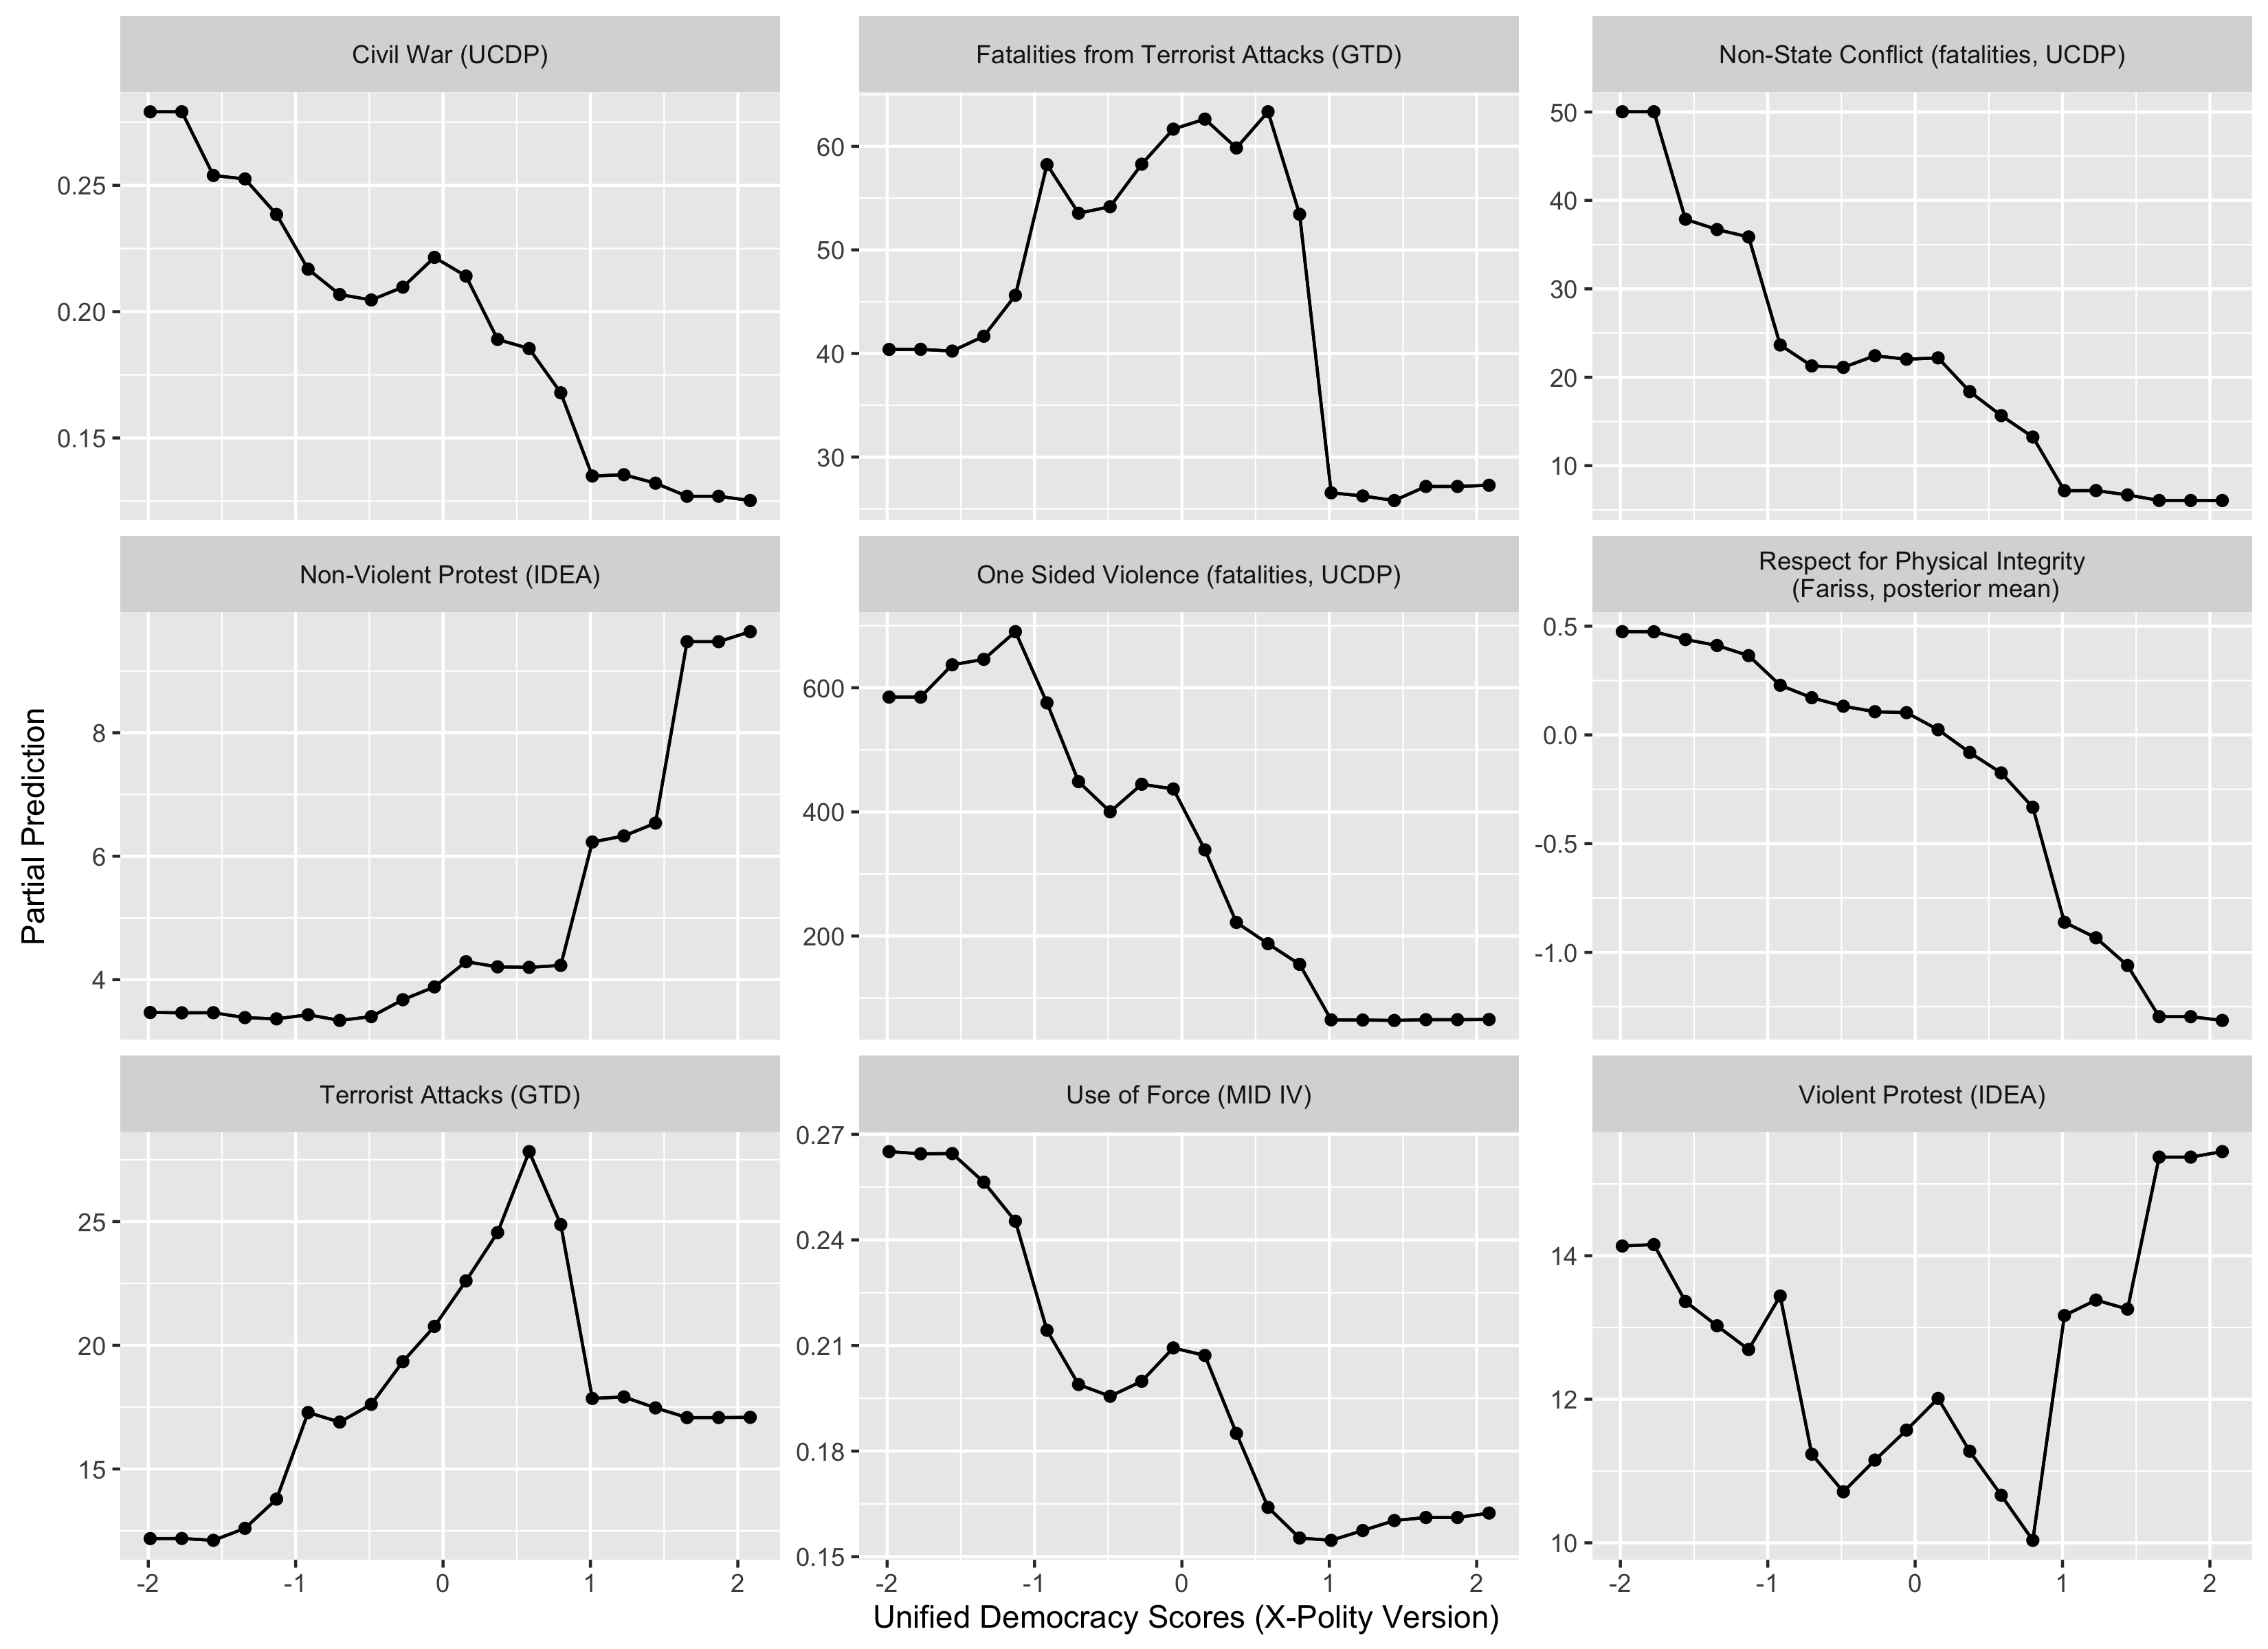
\includegraphics[width=170mm]{../figures/uds_xpolity.png}
\end{center}
\caption{Partial dependence of X-UDS on multiple forms of conflict.}
\label{xuds}
\end{figure}

\begin{figure}[ht!]
\begin{center}
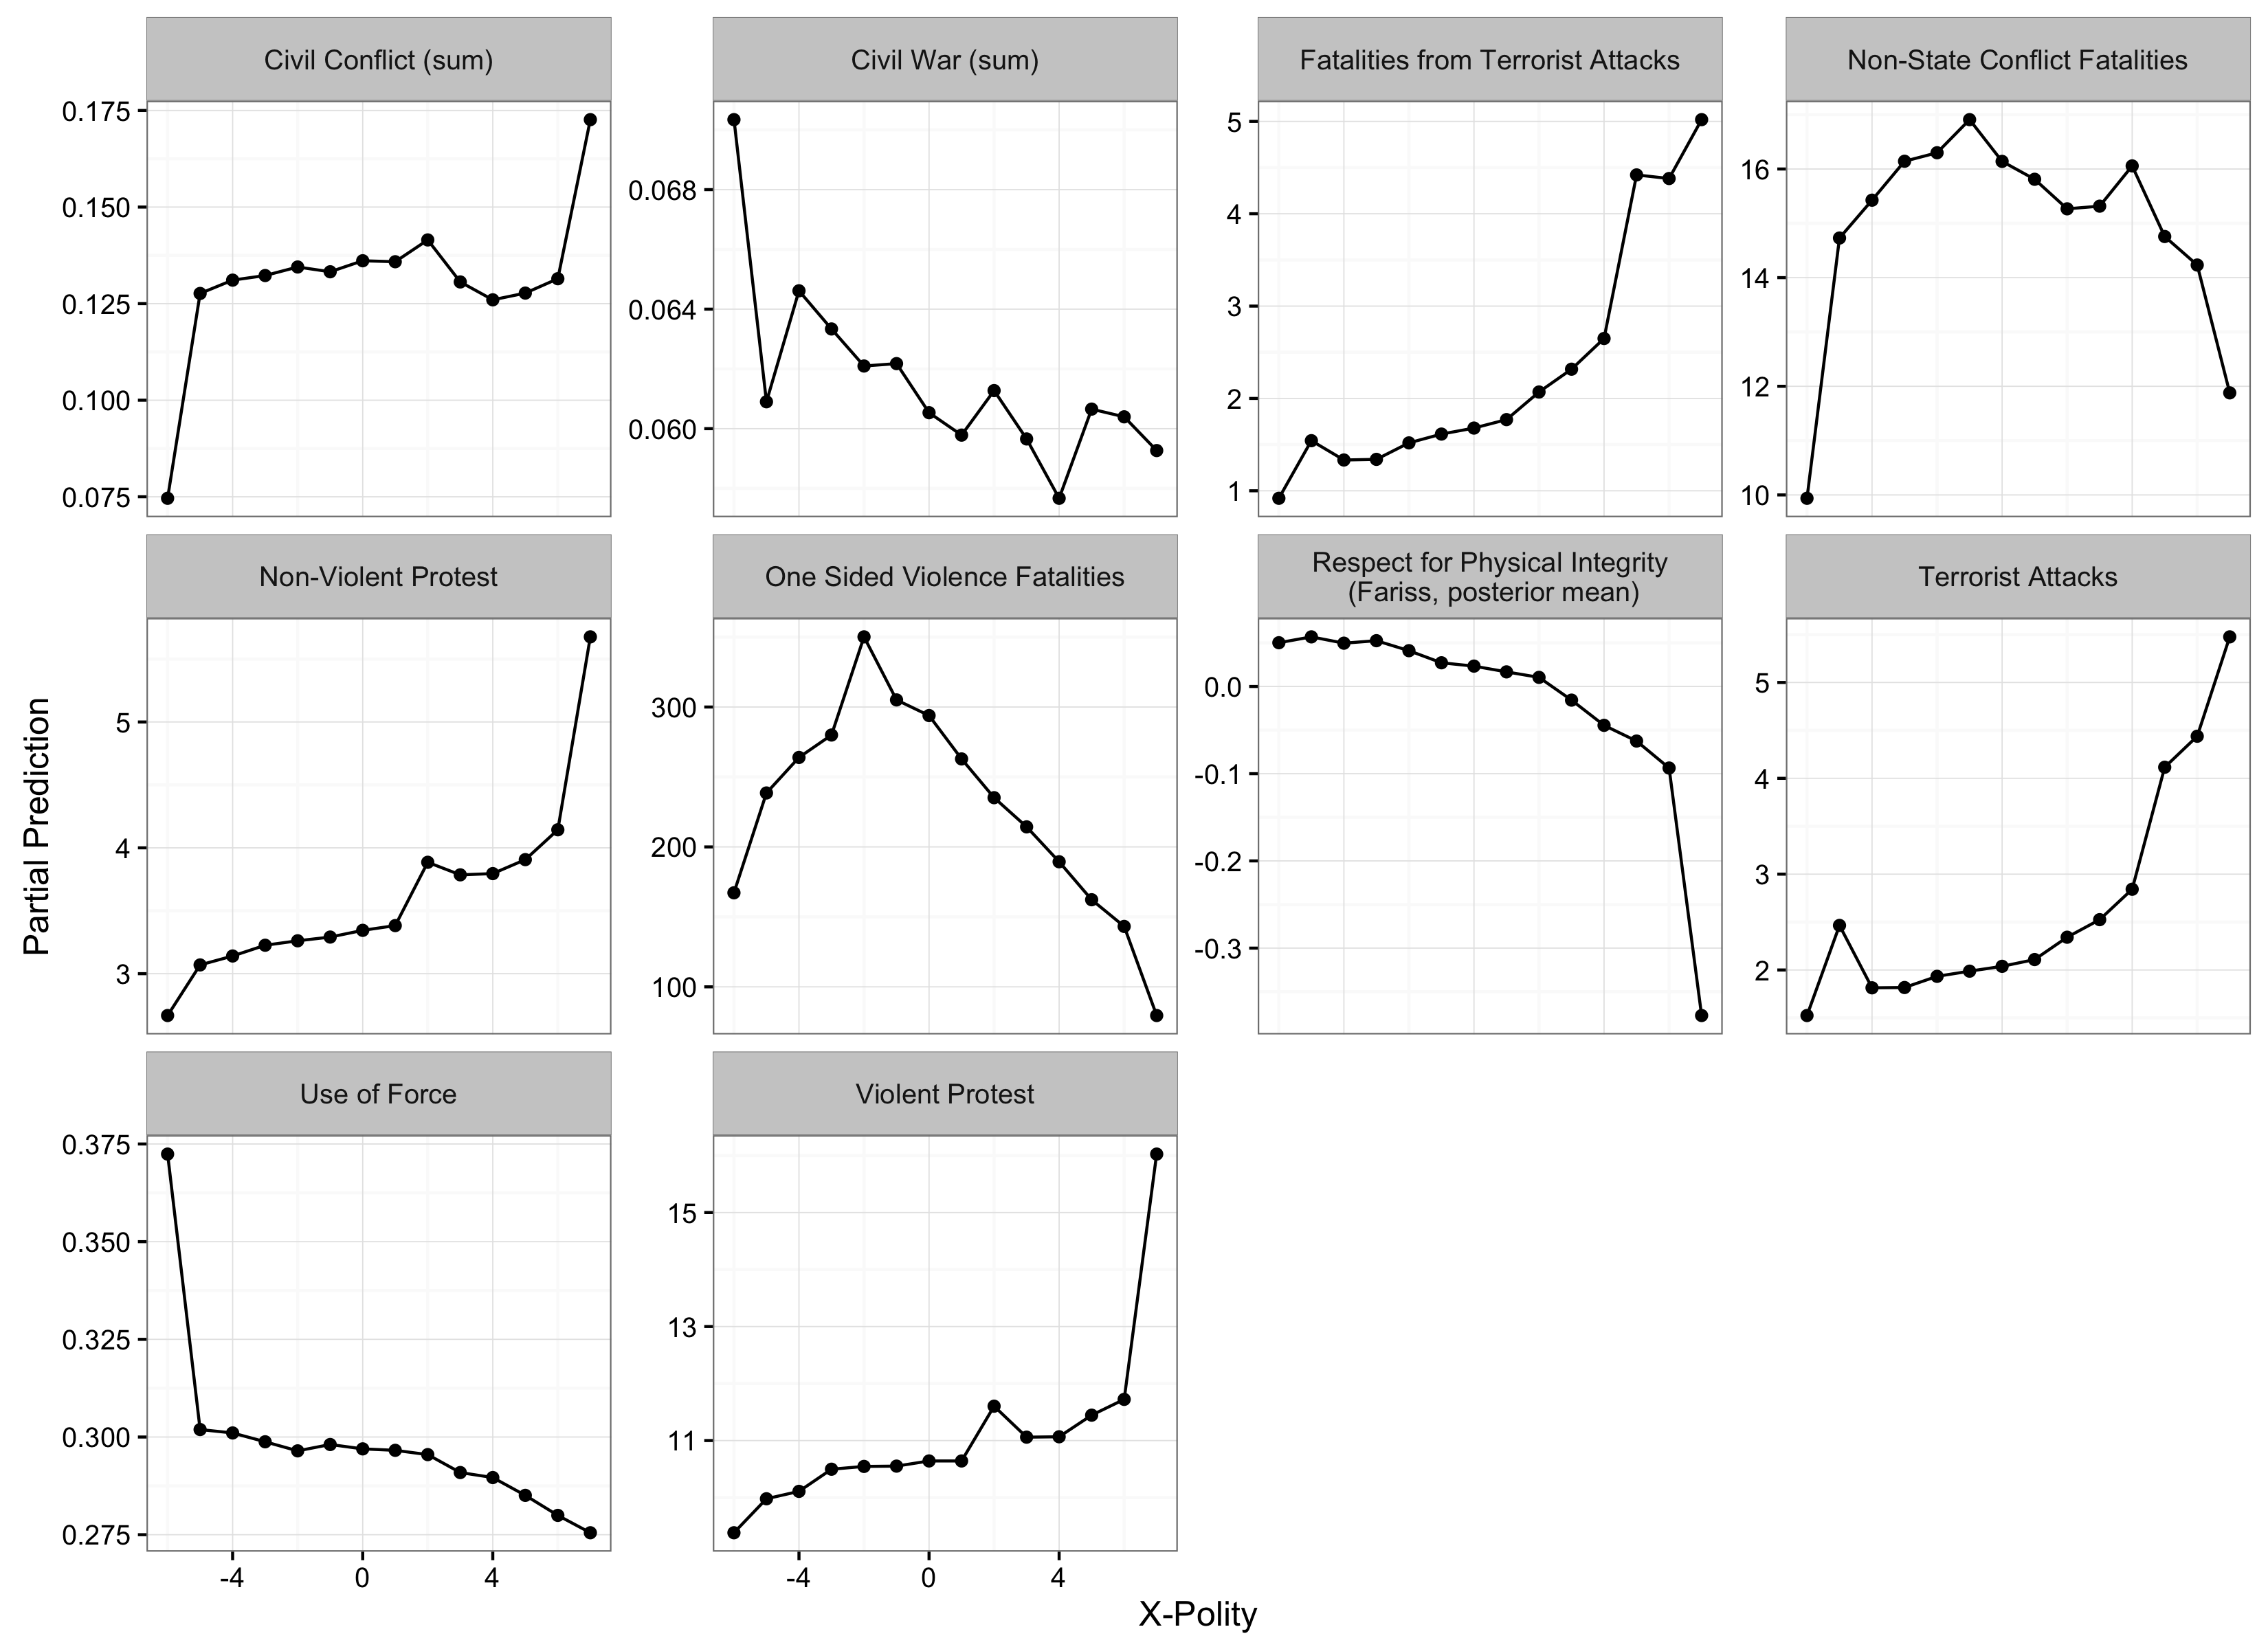
\includegraphics[width=170mm]{../figures/xpolity_nas.png}
\end{center}
\caption{Partial dependence of X-Polity on multiple forms of conflict.}
\label{xpolity}
\end{figure}

\begin{figure}[ht!]
\begin{center}
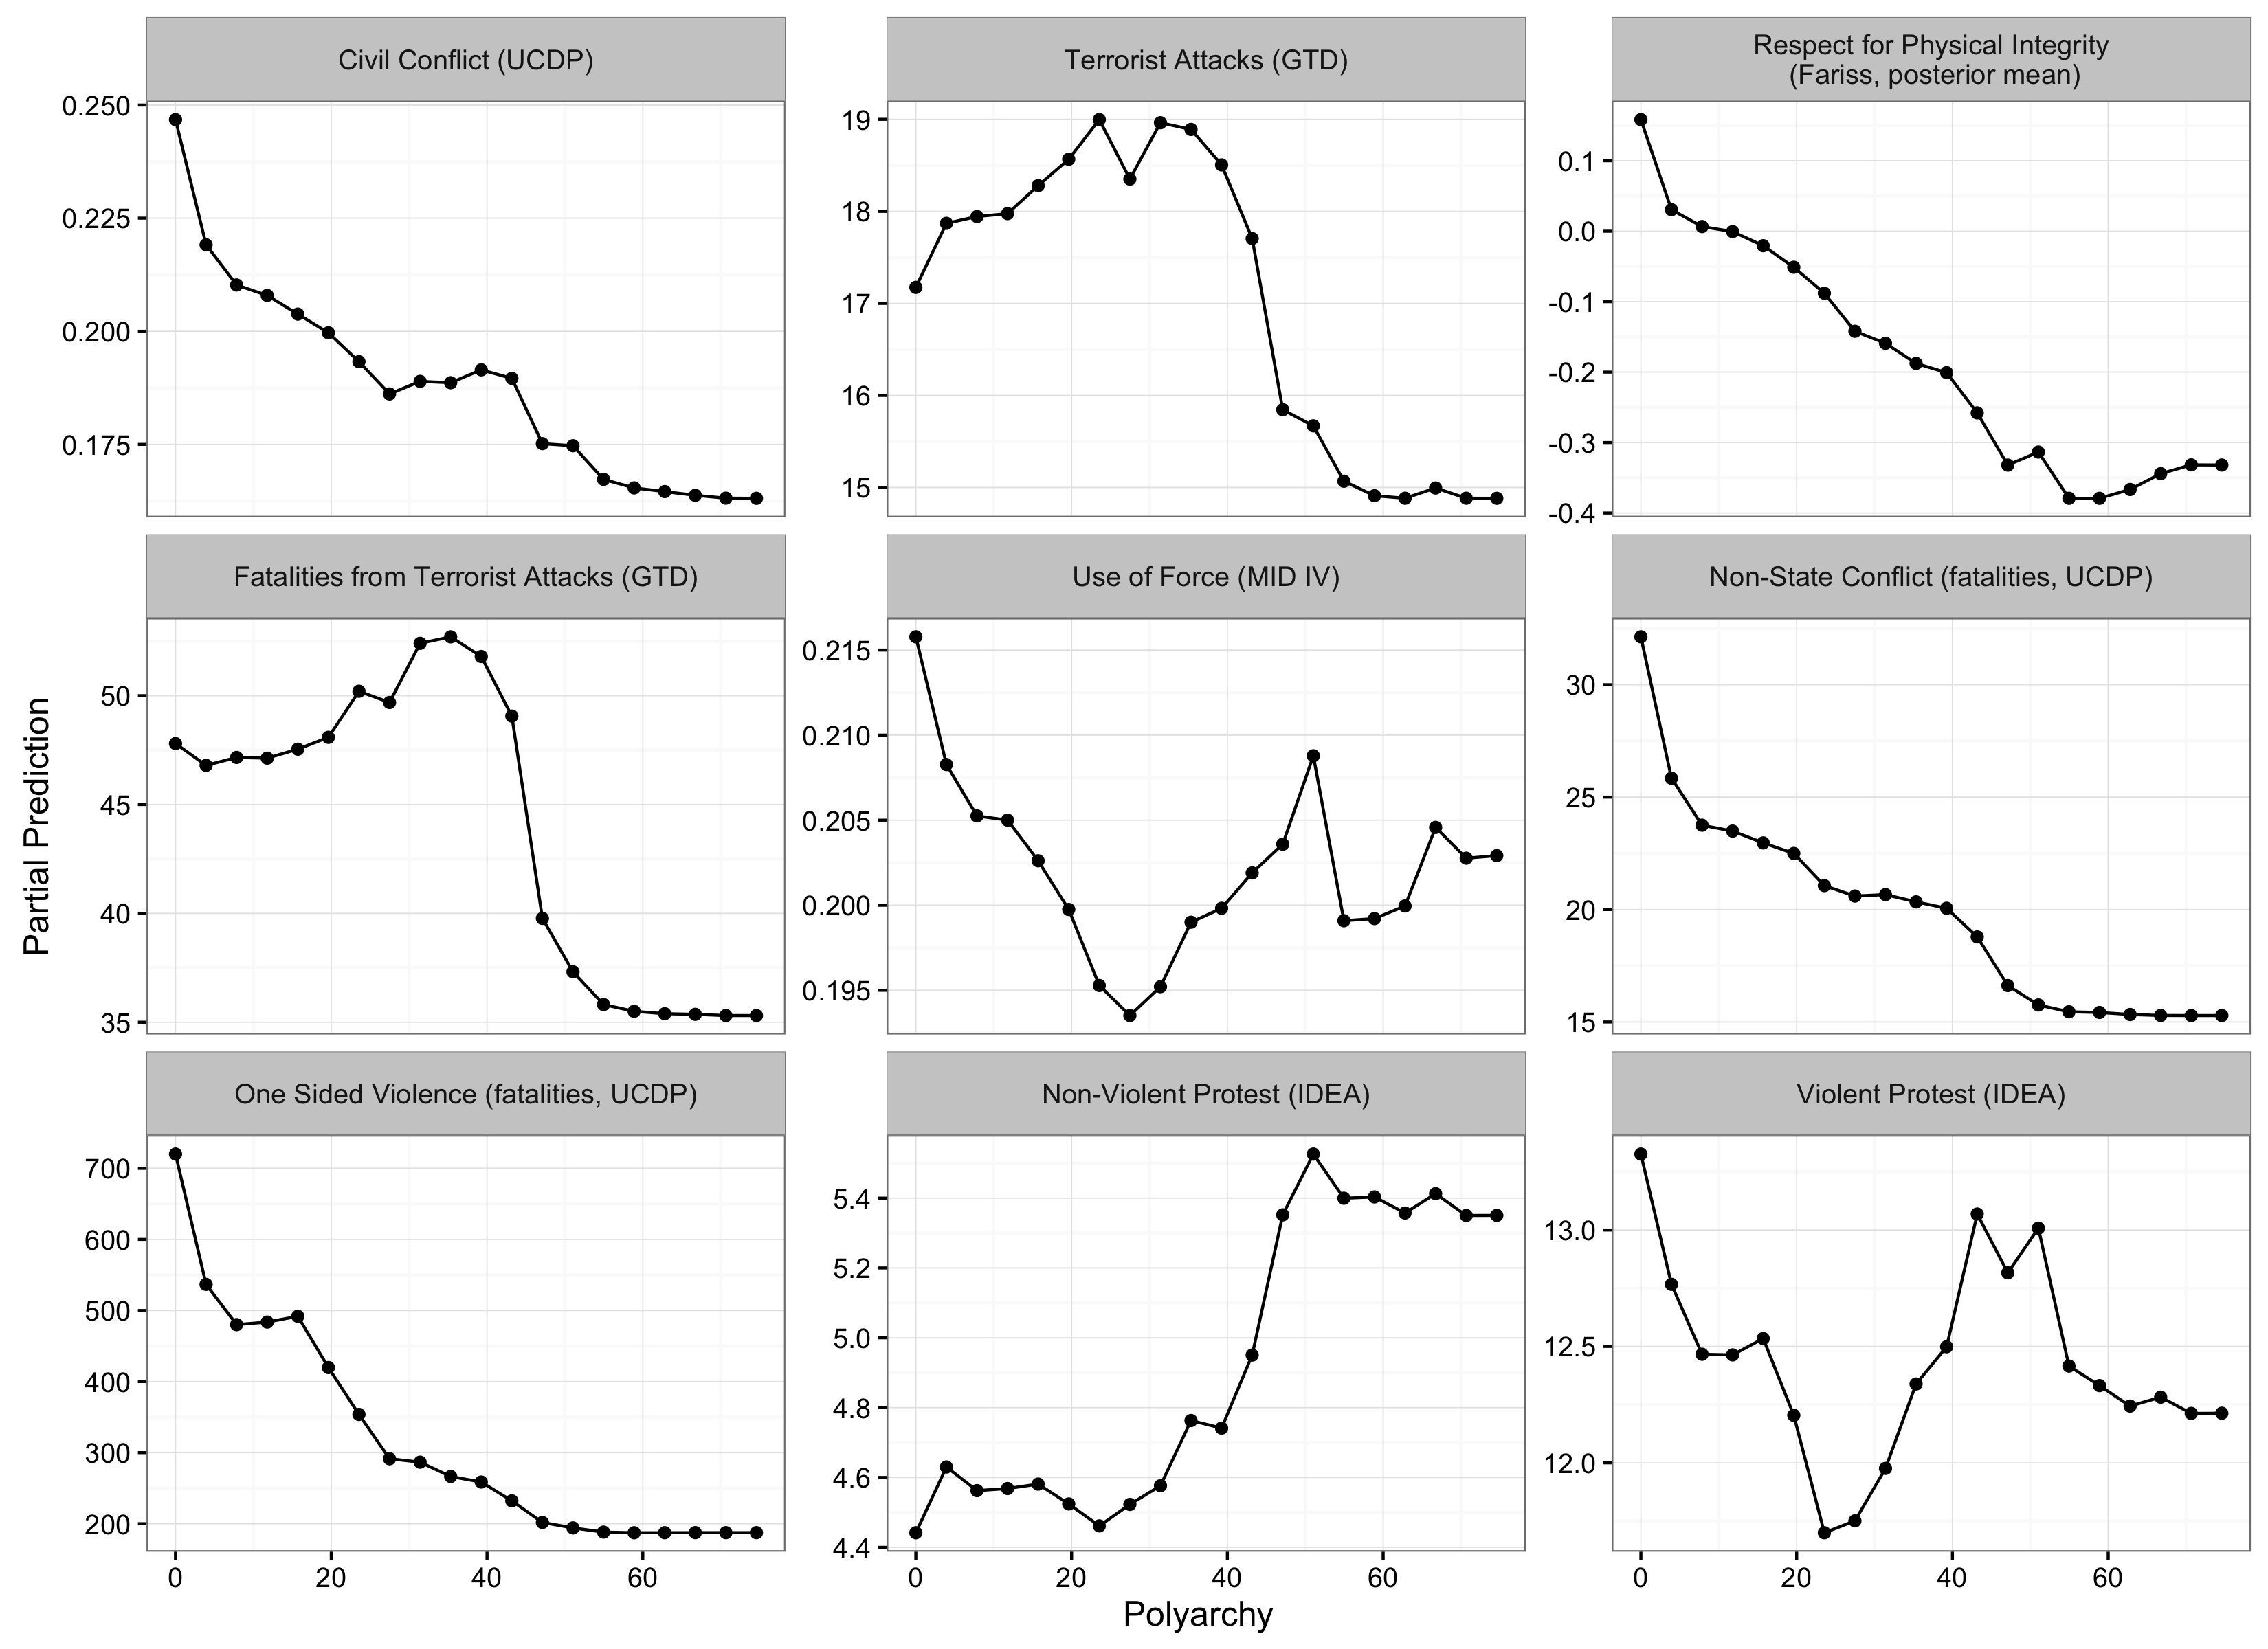
\includegraphics[width=170mm]{../figures/part.png}
\end{center}
\caption{Partial dependence of Participation (Polyarchy) on multiple forms of conflict.}
\label{part}
\end{figure}

\clearpage

Table \ref{results} provides a summary of the extent to which our results are consistent with the MVM Hypothesis.  A ``$+$'' in the table refers to a functional form that follows the inverse-U shape predicted by the MVM Hypothesis, whereas a ``$-$'' refers to a result that does not, most often because the probability of a form of conflict either consistently decreases or increases in more democratic regimes.  In some cases, we refer to a result as ``$(+)$'' because it weakly supports the MVM Hypothesis, e.g., neither democracies nor autocracies face the largest risk of the form of conflict, but the functional form is not quite an inverse-U.

\begin{center}
\begin{table}[h!]
\centering \caption{Support for the MVM Hypothesis}
\bigskip
\label{results}
\normalsize
\begin{tabular}{l c | c |c }
\hline\hline
&\multicolumn{1}{c}{X-UDS}&\multicolumn{1}{c}{X-Polity}&\multicolumn{1}{c}{Polyarchy}\\
\hline\hline
Civil Conflict       & - & + & - \\
Terror Events       & + & - & + \\
Terror Fatalities   & + & - & + \\
Repression          & - & - & - \\
Non-Violent Protests& - & - & - \\
Violent Protests    & - & - & - \\
One-Sided Violence  & (+) & (+)& - \\
Non-State Conflict  & - & + & - \\
Use of Force (MID)  & - & - & - \\
\hline\hline
\end{tabular}
\end{table}
\end{center}

\subsection{Regime Type and Conflict over Time}

Our results also indicate the extent to which the relationships between regime type and conflict have evolved over time.  We represent these results by using a series of heat maps.  In each heat map, the x-axis represents a measure of regime type, and the y-axis represents time.  Each square in the heat map represents the partial prediction with respect to the applicable regime type level, conflict type, and year.  Squares in darker red indicate that the risk of that form of conflict in that type of regime in that year was larger.

Figures \ref{xuds_cwar}, \ref{xpolity_cwar}, and \ref{part_cwar} provide the heat maps of civil conflict risk from our models using X-UDS, X-Polity, and Polyarchy, respectively.  An interesting observation that emerges from these plots is that there appears to be a significant structural change in the data at the end of the Cold War, i.e., the risks of civil conflict at individual regime types changed relatively little throughout the 1980s, changed significantly in 1990, and have again changed relatively little since then.  This is consistent with evidence that suggests civil conflicts during the Cold War had different characteristics than post-Cold War civil conflicts \citep{kalyvas2001new}.  An additional observation is that the support for the MVM Hypothesis using the X-Polity data shown in Figure \ref{xpolity} may be driven largely by the post-Cold War era.  As Figure \ref{xpolity_cwar} indicates, the risk of civil conflicts was largest in the most democratic states along the X-polity scale during the Cold War, but has since changed to being in the middle range of the scale.

\clearpage

\begin{figure}[ht!]
\begin{center}
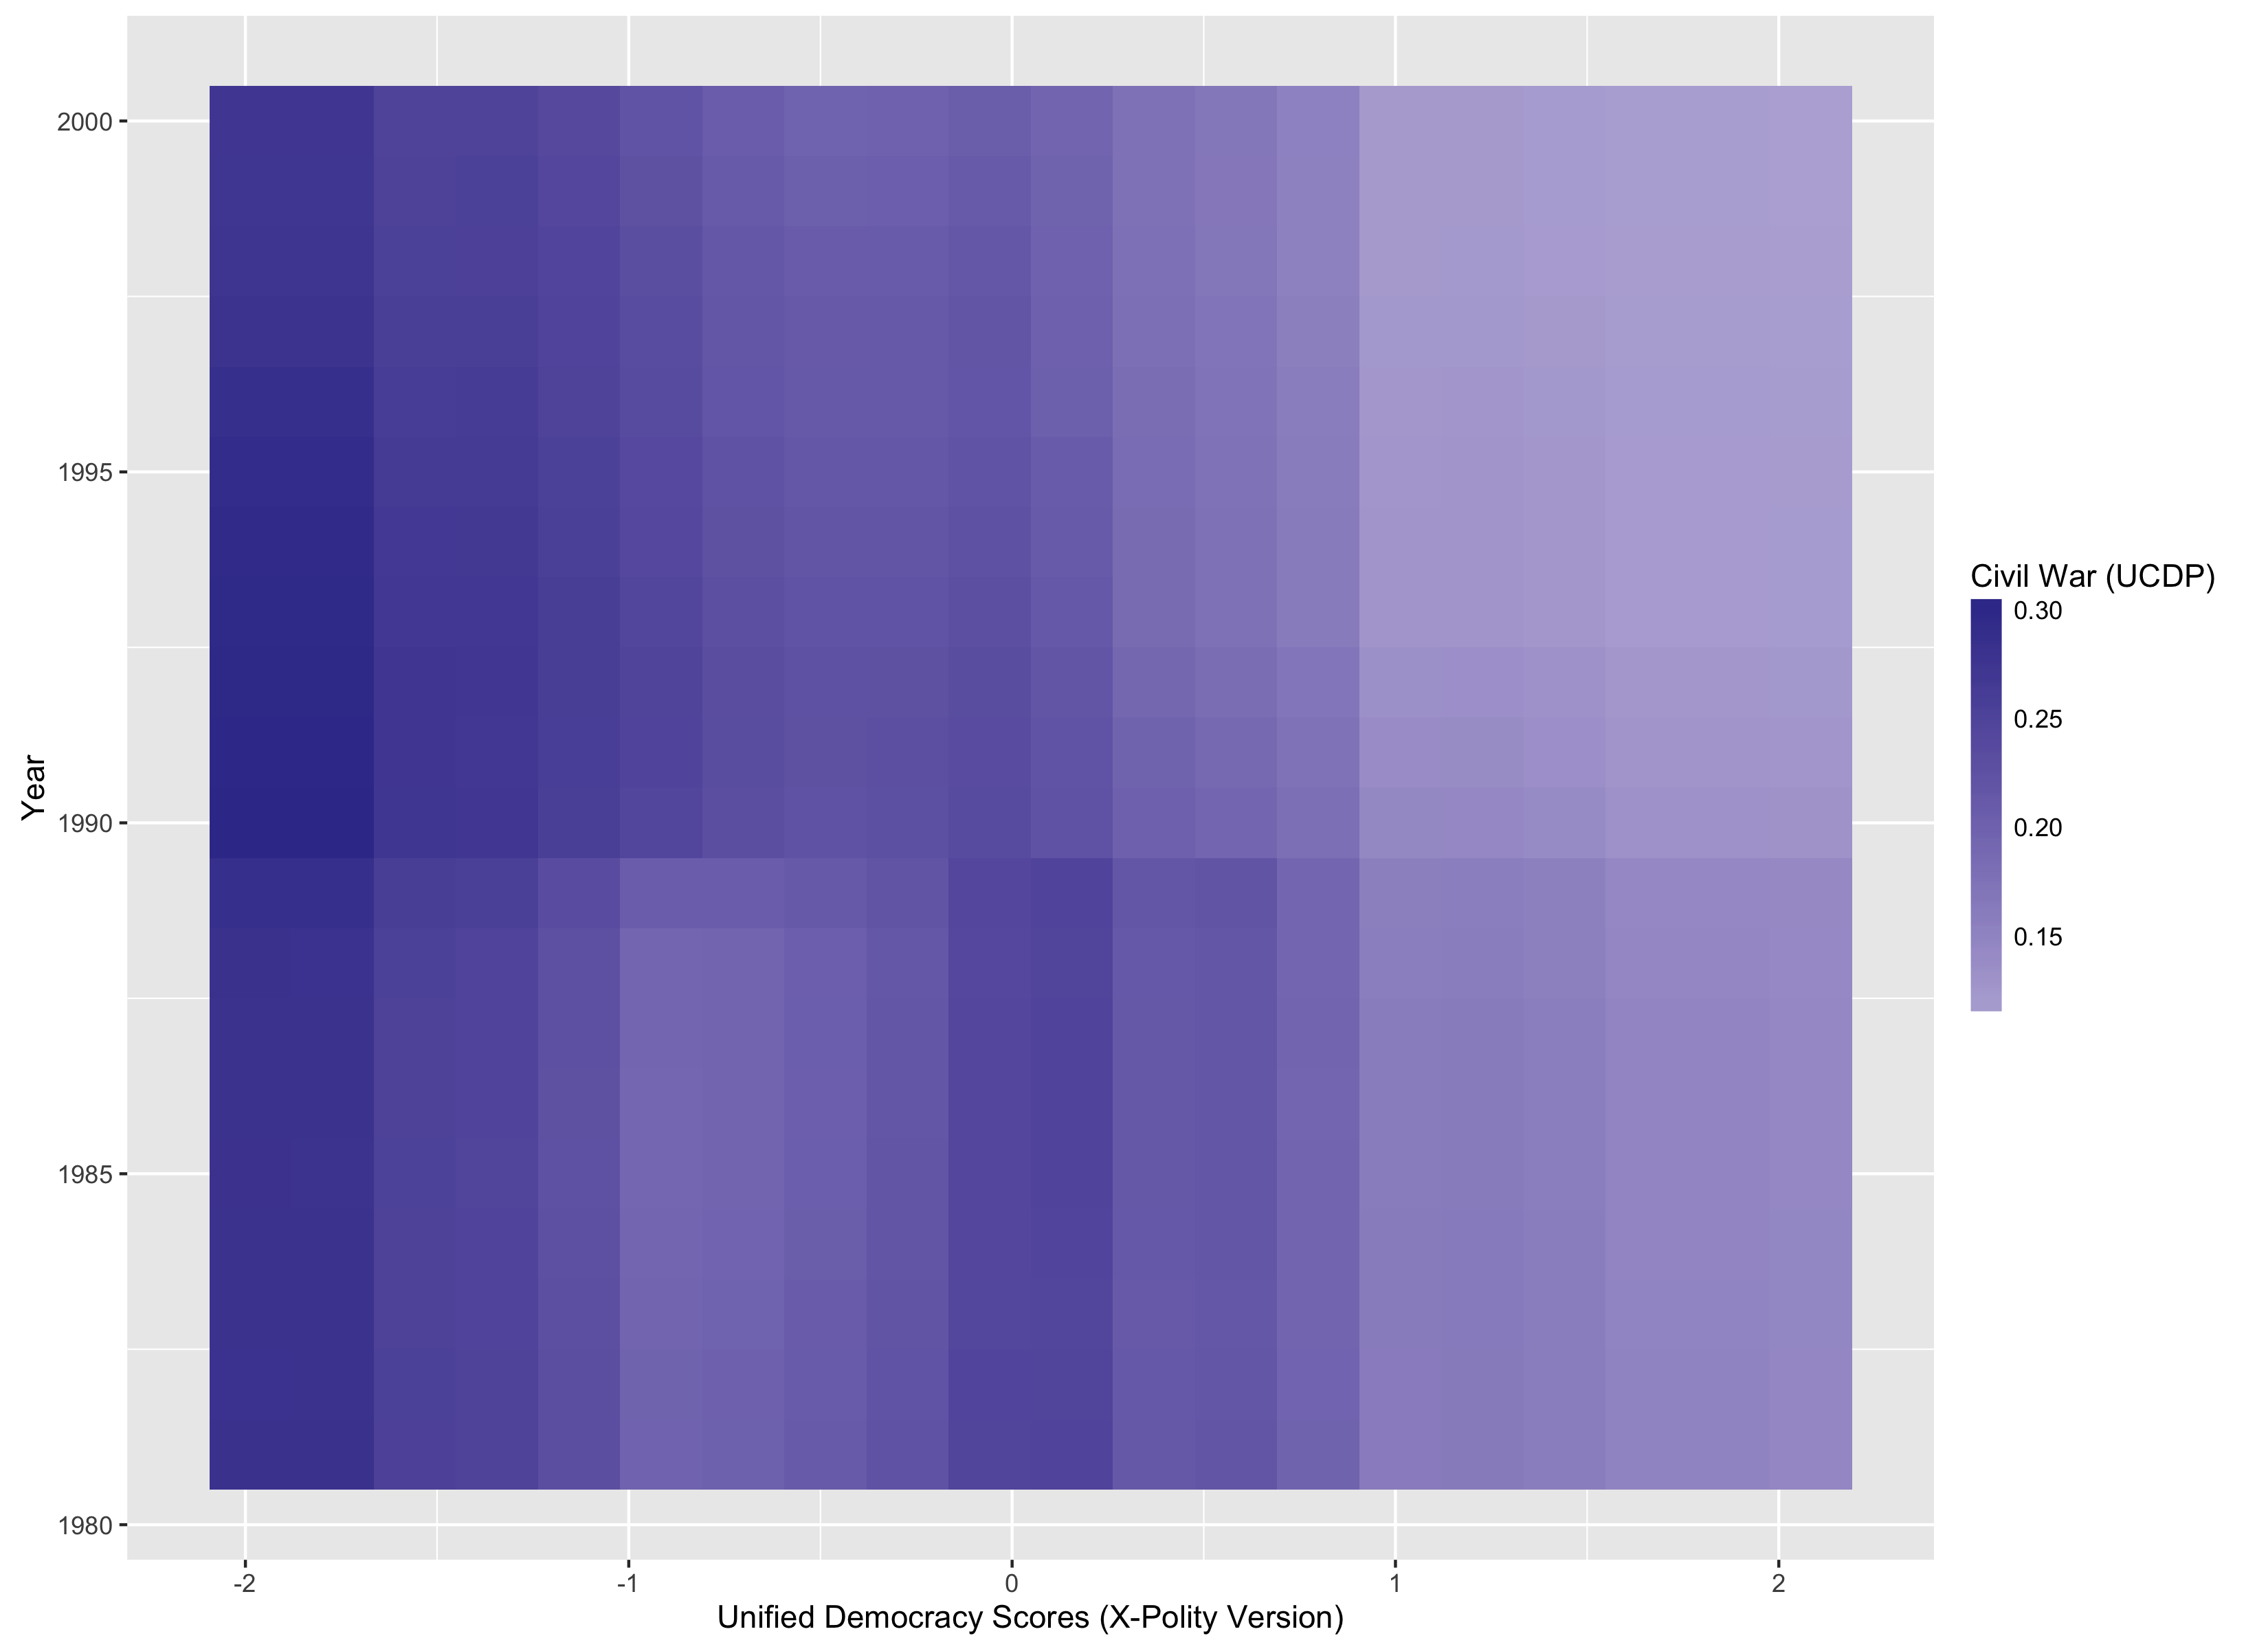
\includegraphics[width=100mm]{../figures/cwar_uds_xpolity_int_year_tile.png}
\end{center}
\caption{Partial dependence of X-UDS on Civil Conflict over Time}
\label{xuds_cwar}
\end{figure}

\begin{figure}[h!]
\begin{center}
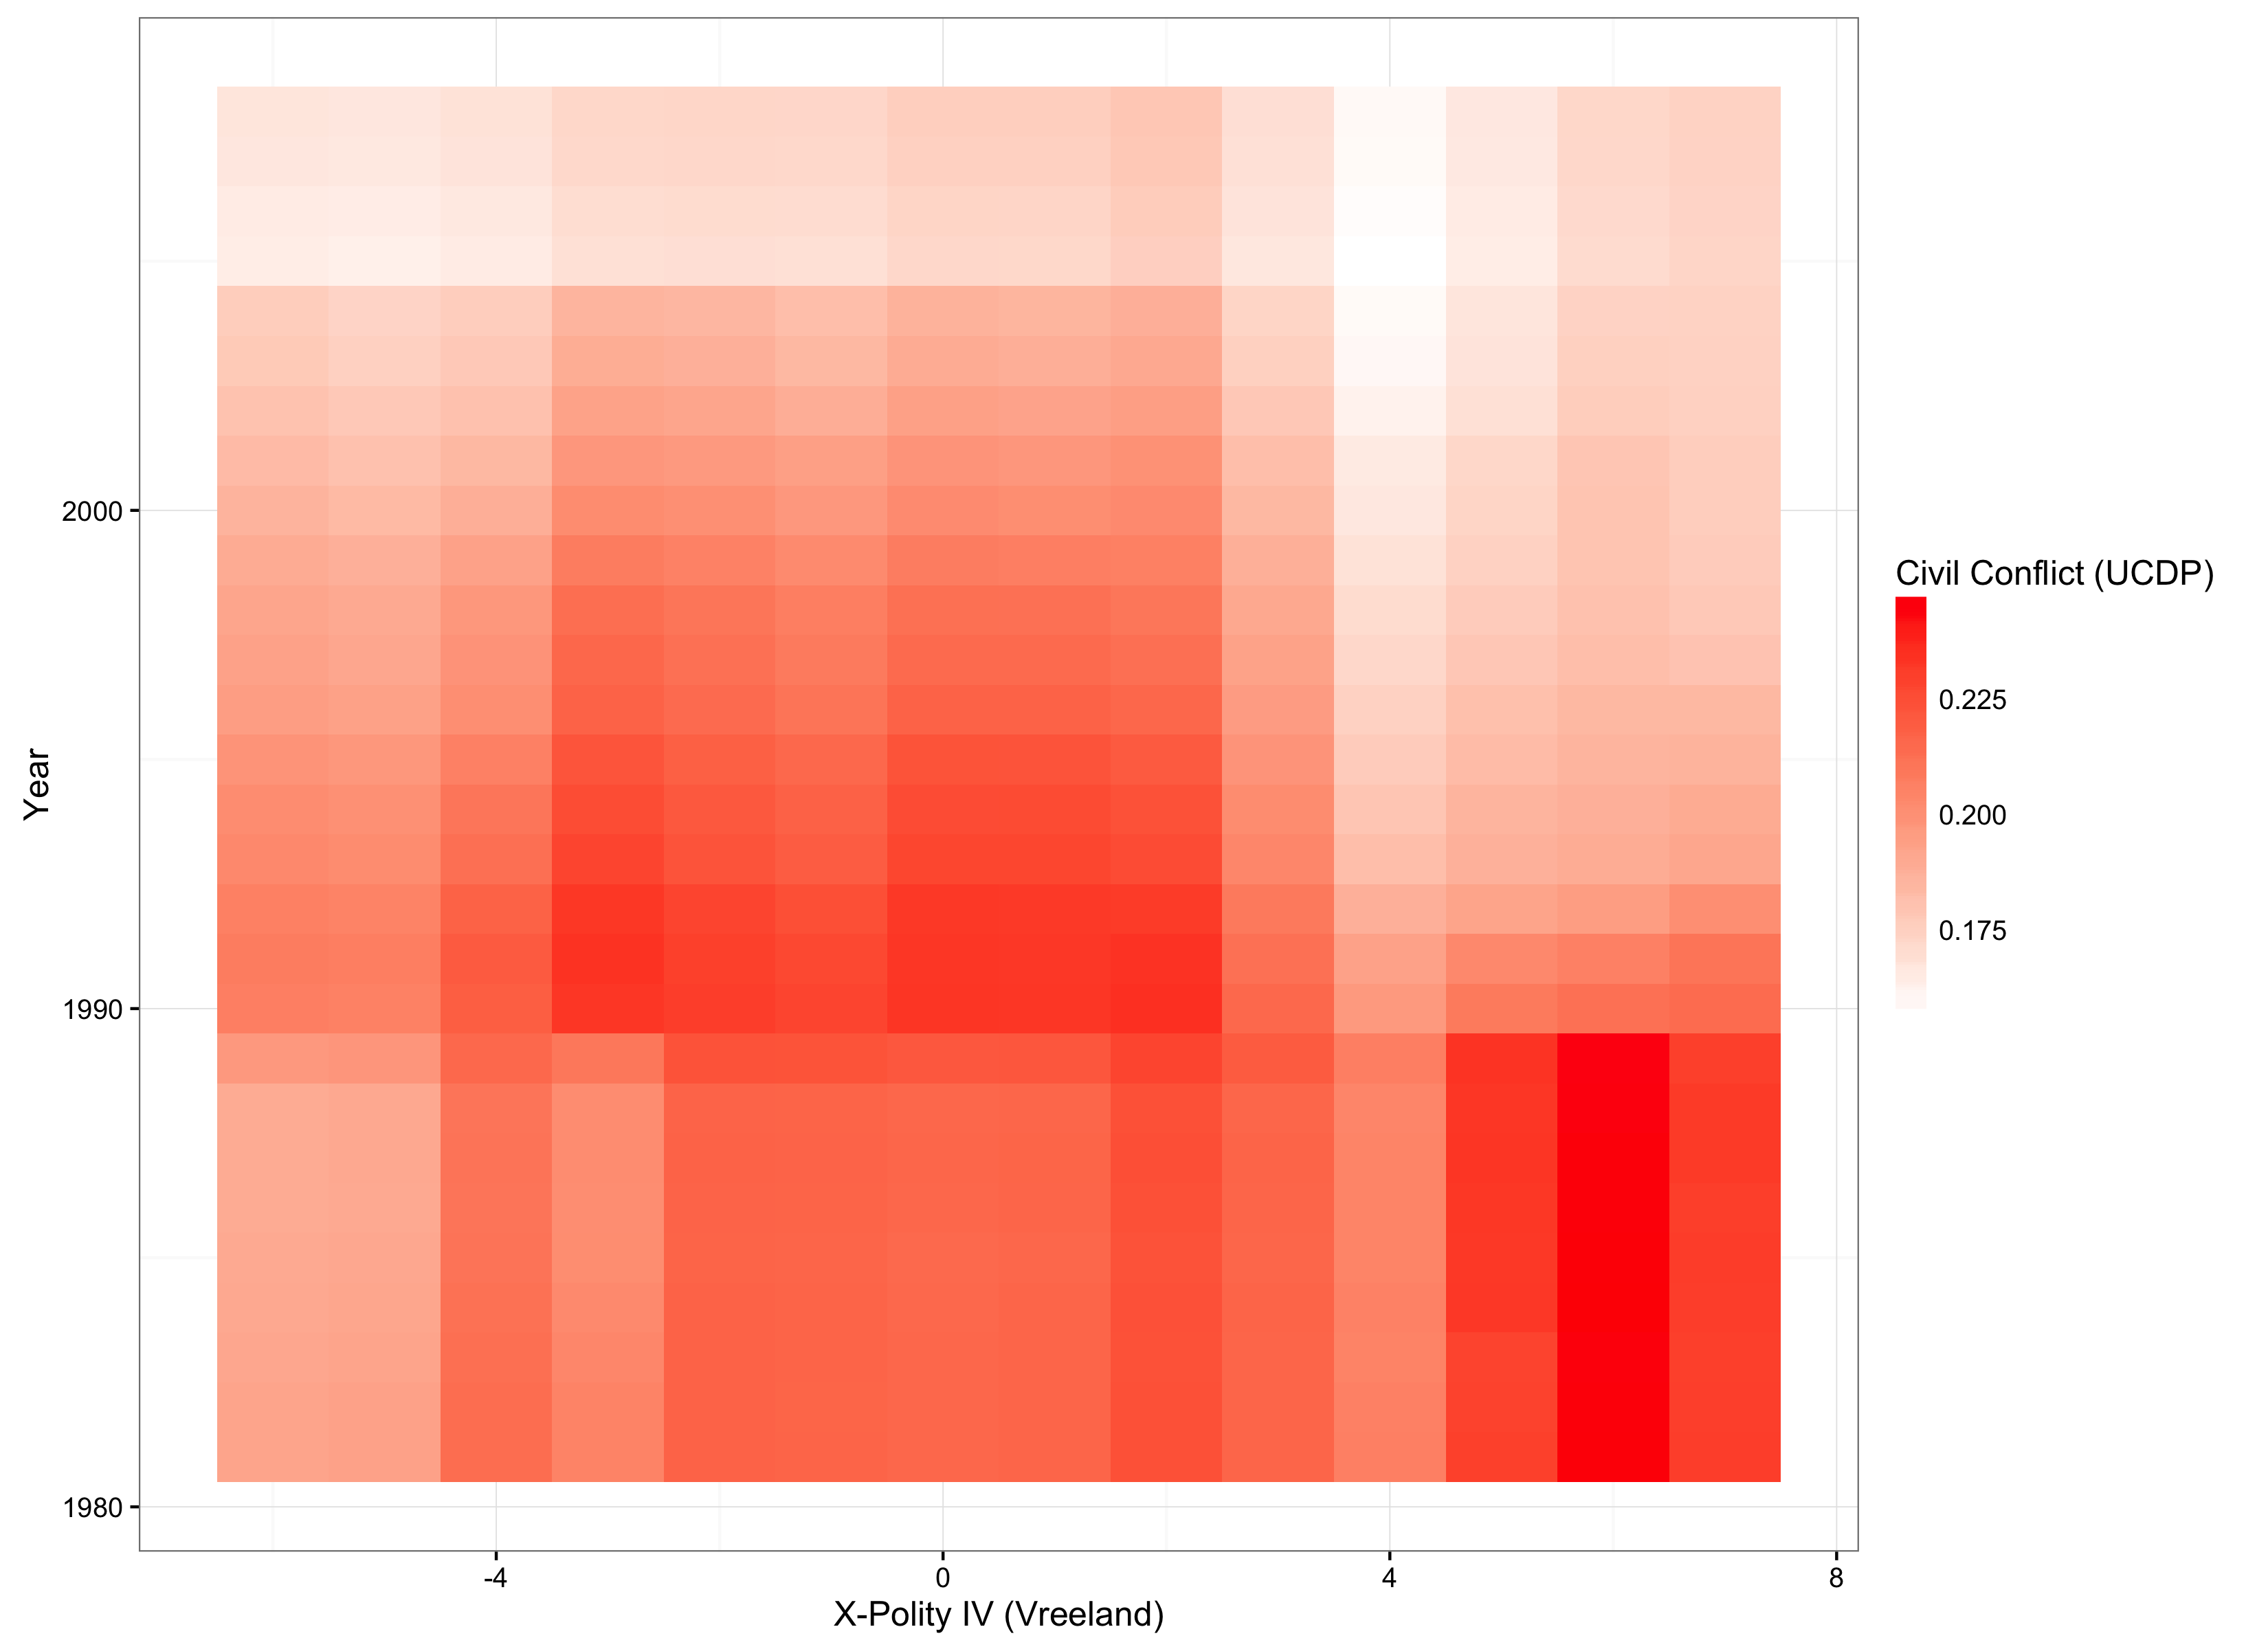
\includegraphics[width=100mm]{../figures/cwar_xpolity_nas_int_year_tile.png}
\end{center}
\caption{Partial dependence of X-Polity on Civil Conflict over Time}
\label{xpolity_cwar}
\end{figure}

\clearpage

\begin{figure}[ht!]
\begin{center}
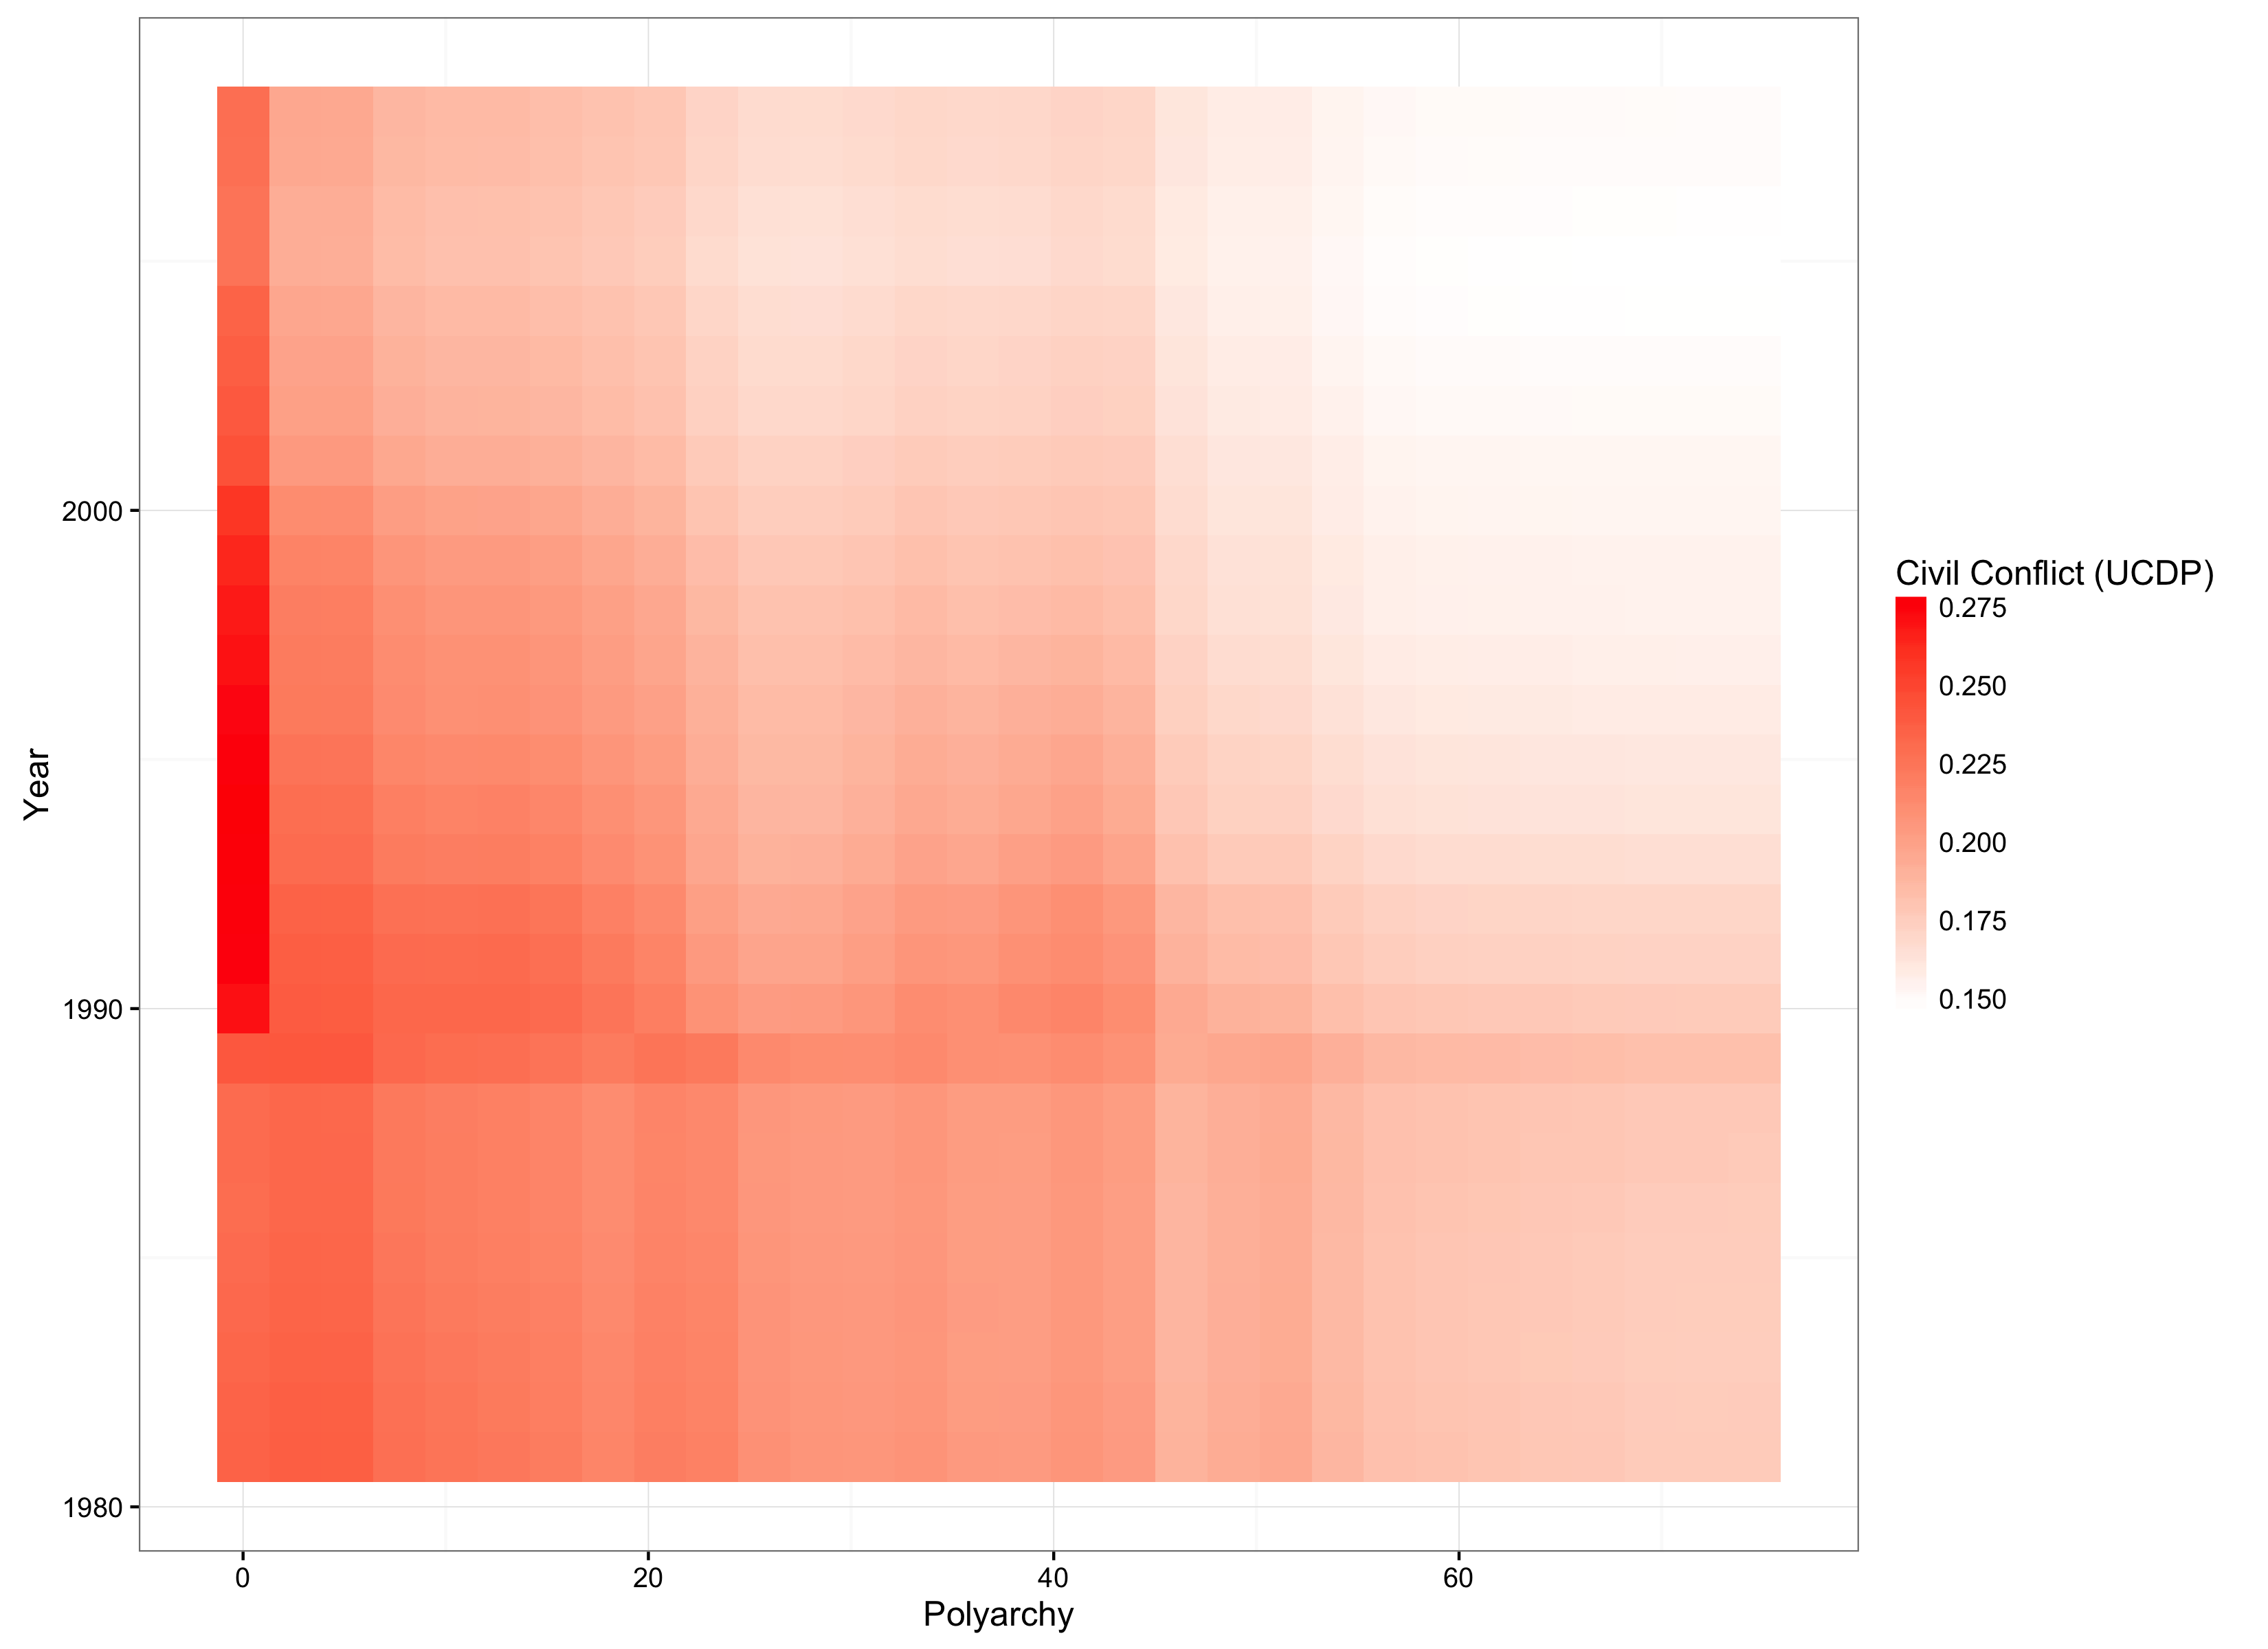
\includegraphics[width=100mm]{../figures/cwar_part_int_year_tile.png}
\end{center}
\caption{Partial dependence of Participation on Civil Conflict over Time}
\label{part_cwar}
\end{figure}

Figures \ref{xuds_rep}, \ref{xpolity_rep}, and \ref{part_rep} provide the heat maps of the risk of physical integrity rights repression from our models using X-UDS, X-Polity, and Polyarchy, respectively.  Several observations are worth noting with respect to these heat maps.  First, there do appear be major differences with respect to the regime type-repression relationship over time.  Across all measures of regime type and all years, we find that the most autocratic regimes are also the most likely to abuse physical integrity rights.  Second, the overall risk of repression appears to decrease in later years in data, which supports \citeauthor{fariss2014respect}'s (\citeyear{fariss2014respect}) finding.  The largest decrease in the risk of repression appears to occur at the end of the Cold War, which is also consistent with \citeauthor{fariss2014respect}'s (\citeyear{fariss2014respect}) result.

\clearpage

\begin{figure}[ht!]
\begin{center}
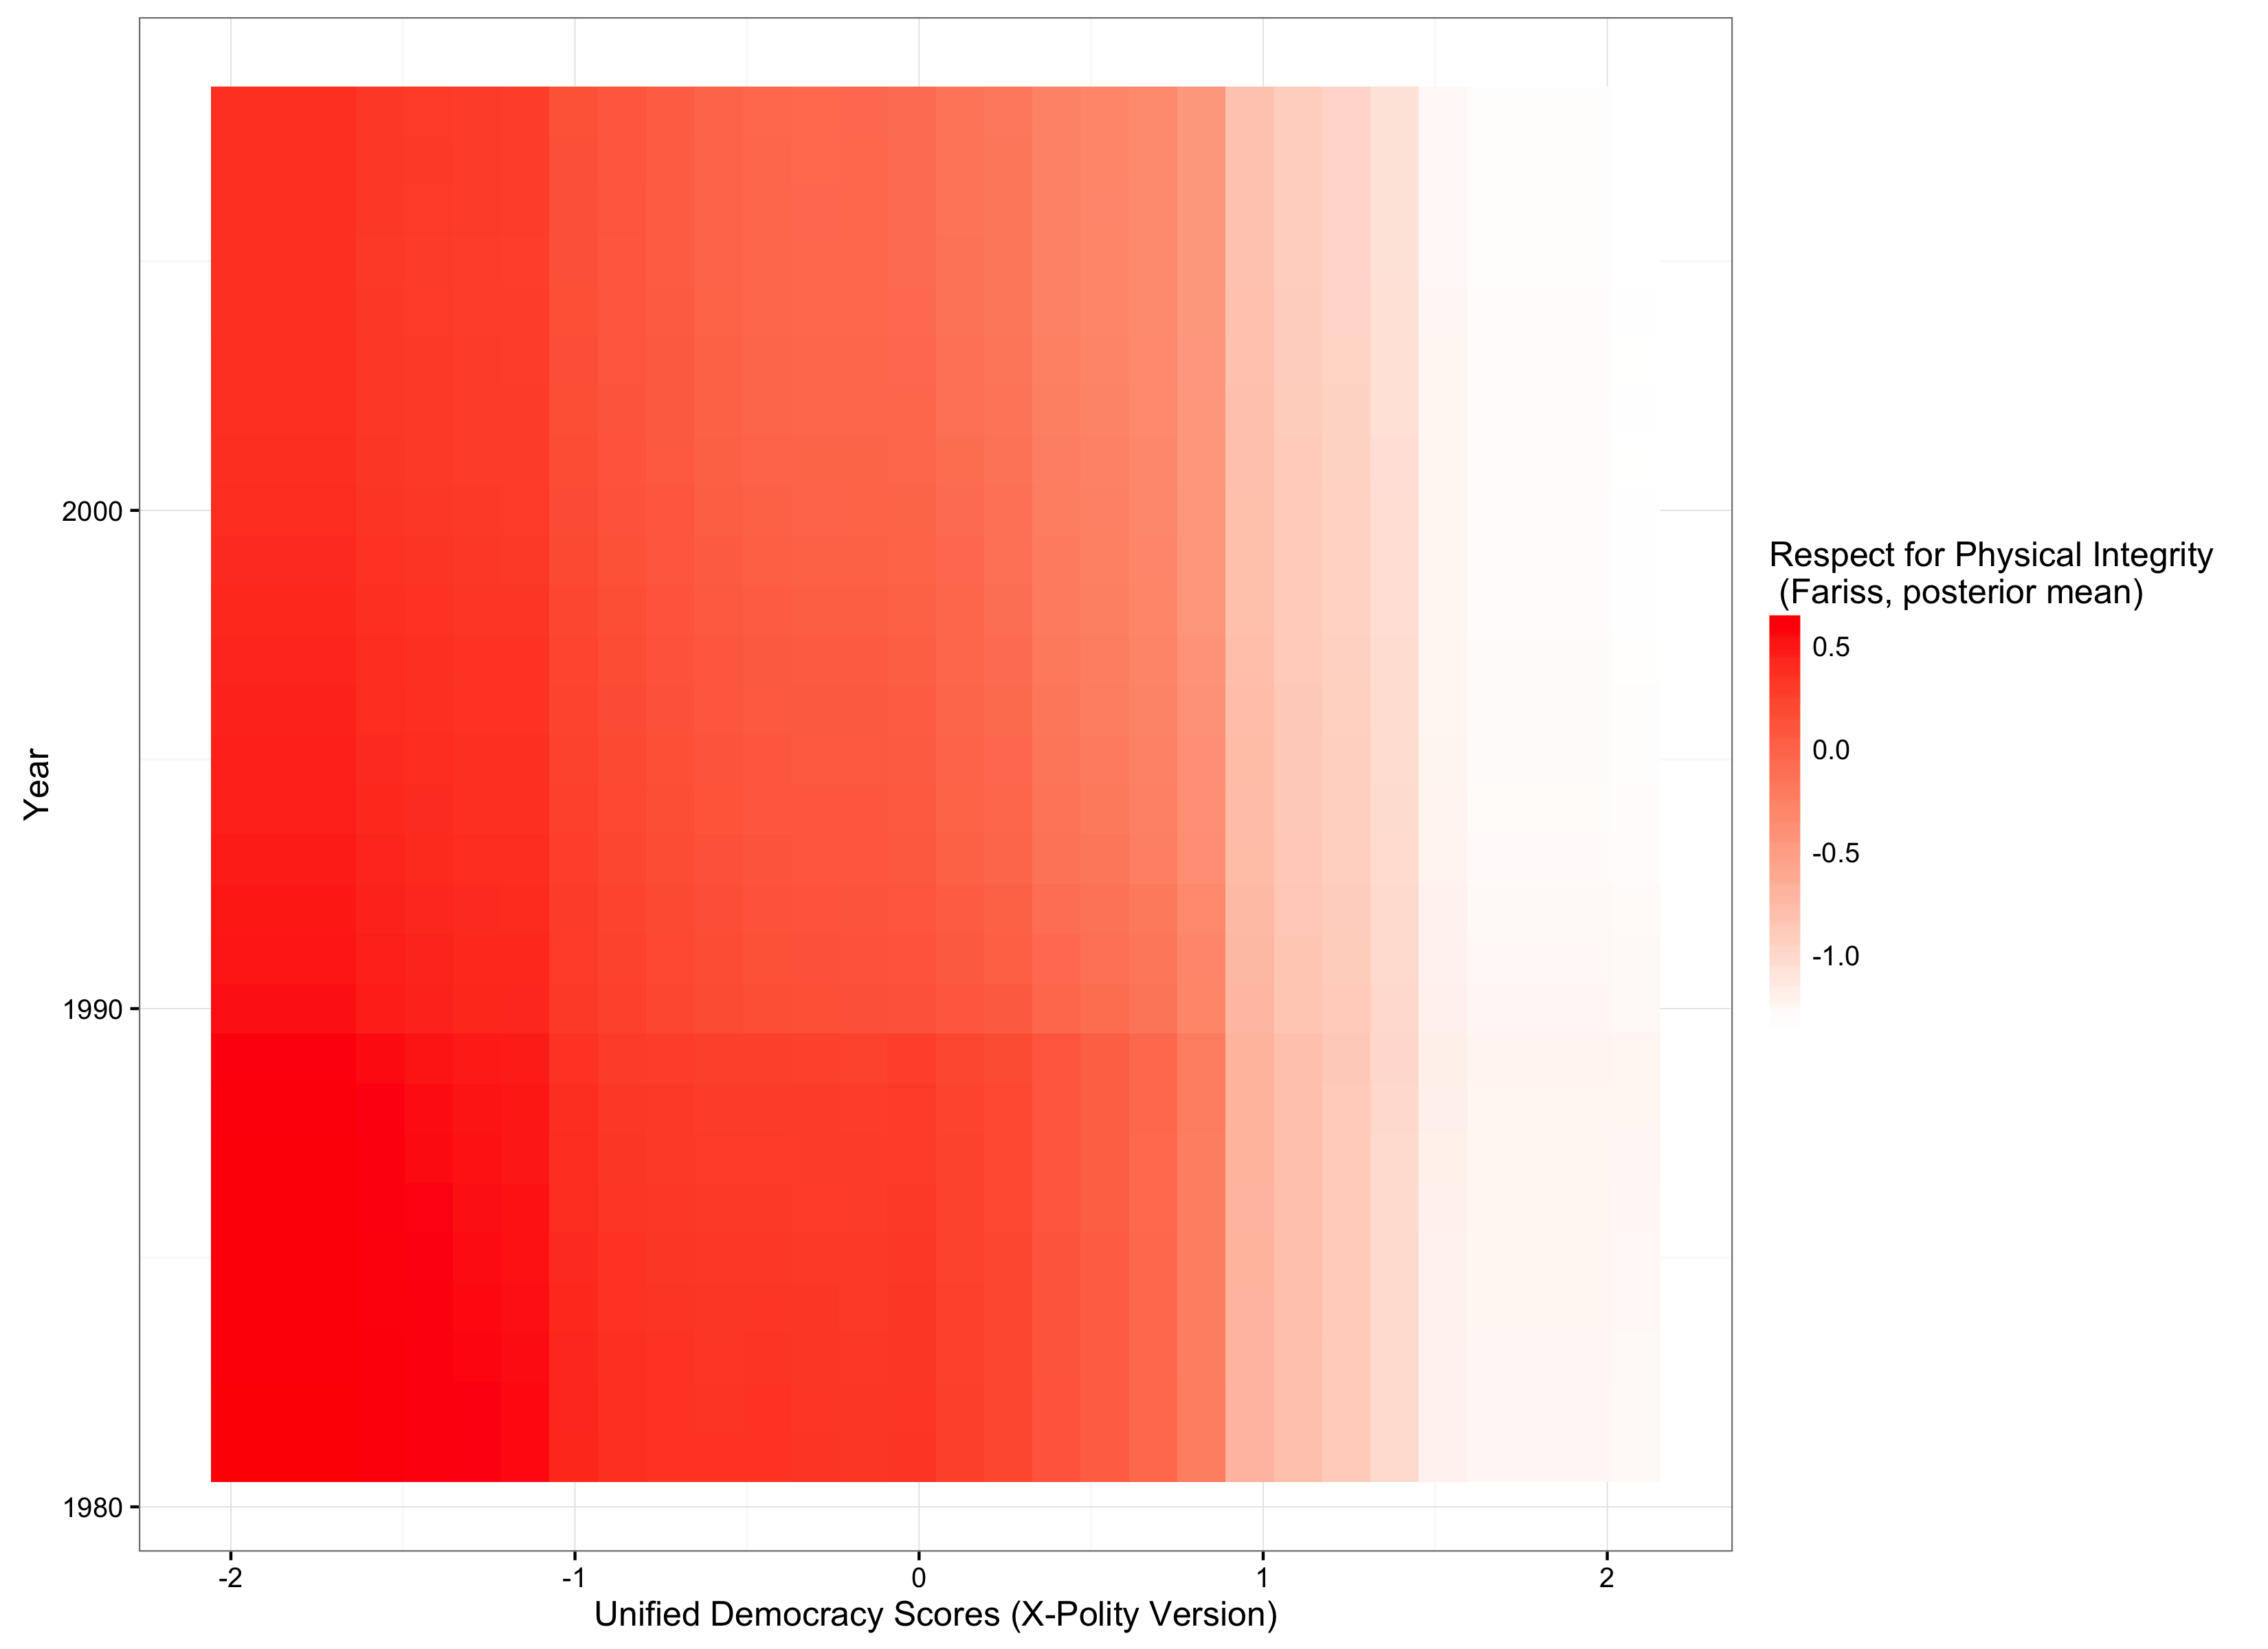
\includegraphics[width=100mm]{../figures/latent_mean_uds_xpolity_int_year_tile.png}
\end{center}
\caption{Partial dependence of X-UDS on Repression over Time.}
\label{xuds_rep}
\end{figure}

\begin{figure}[h!]
\begin{center}
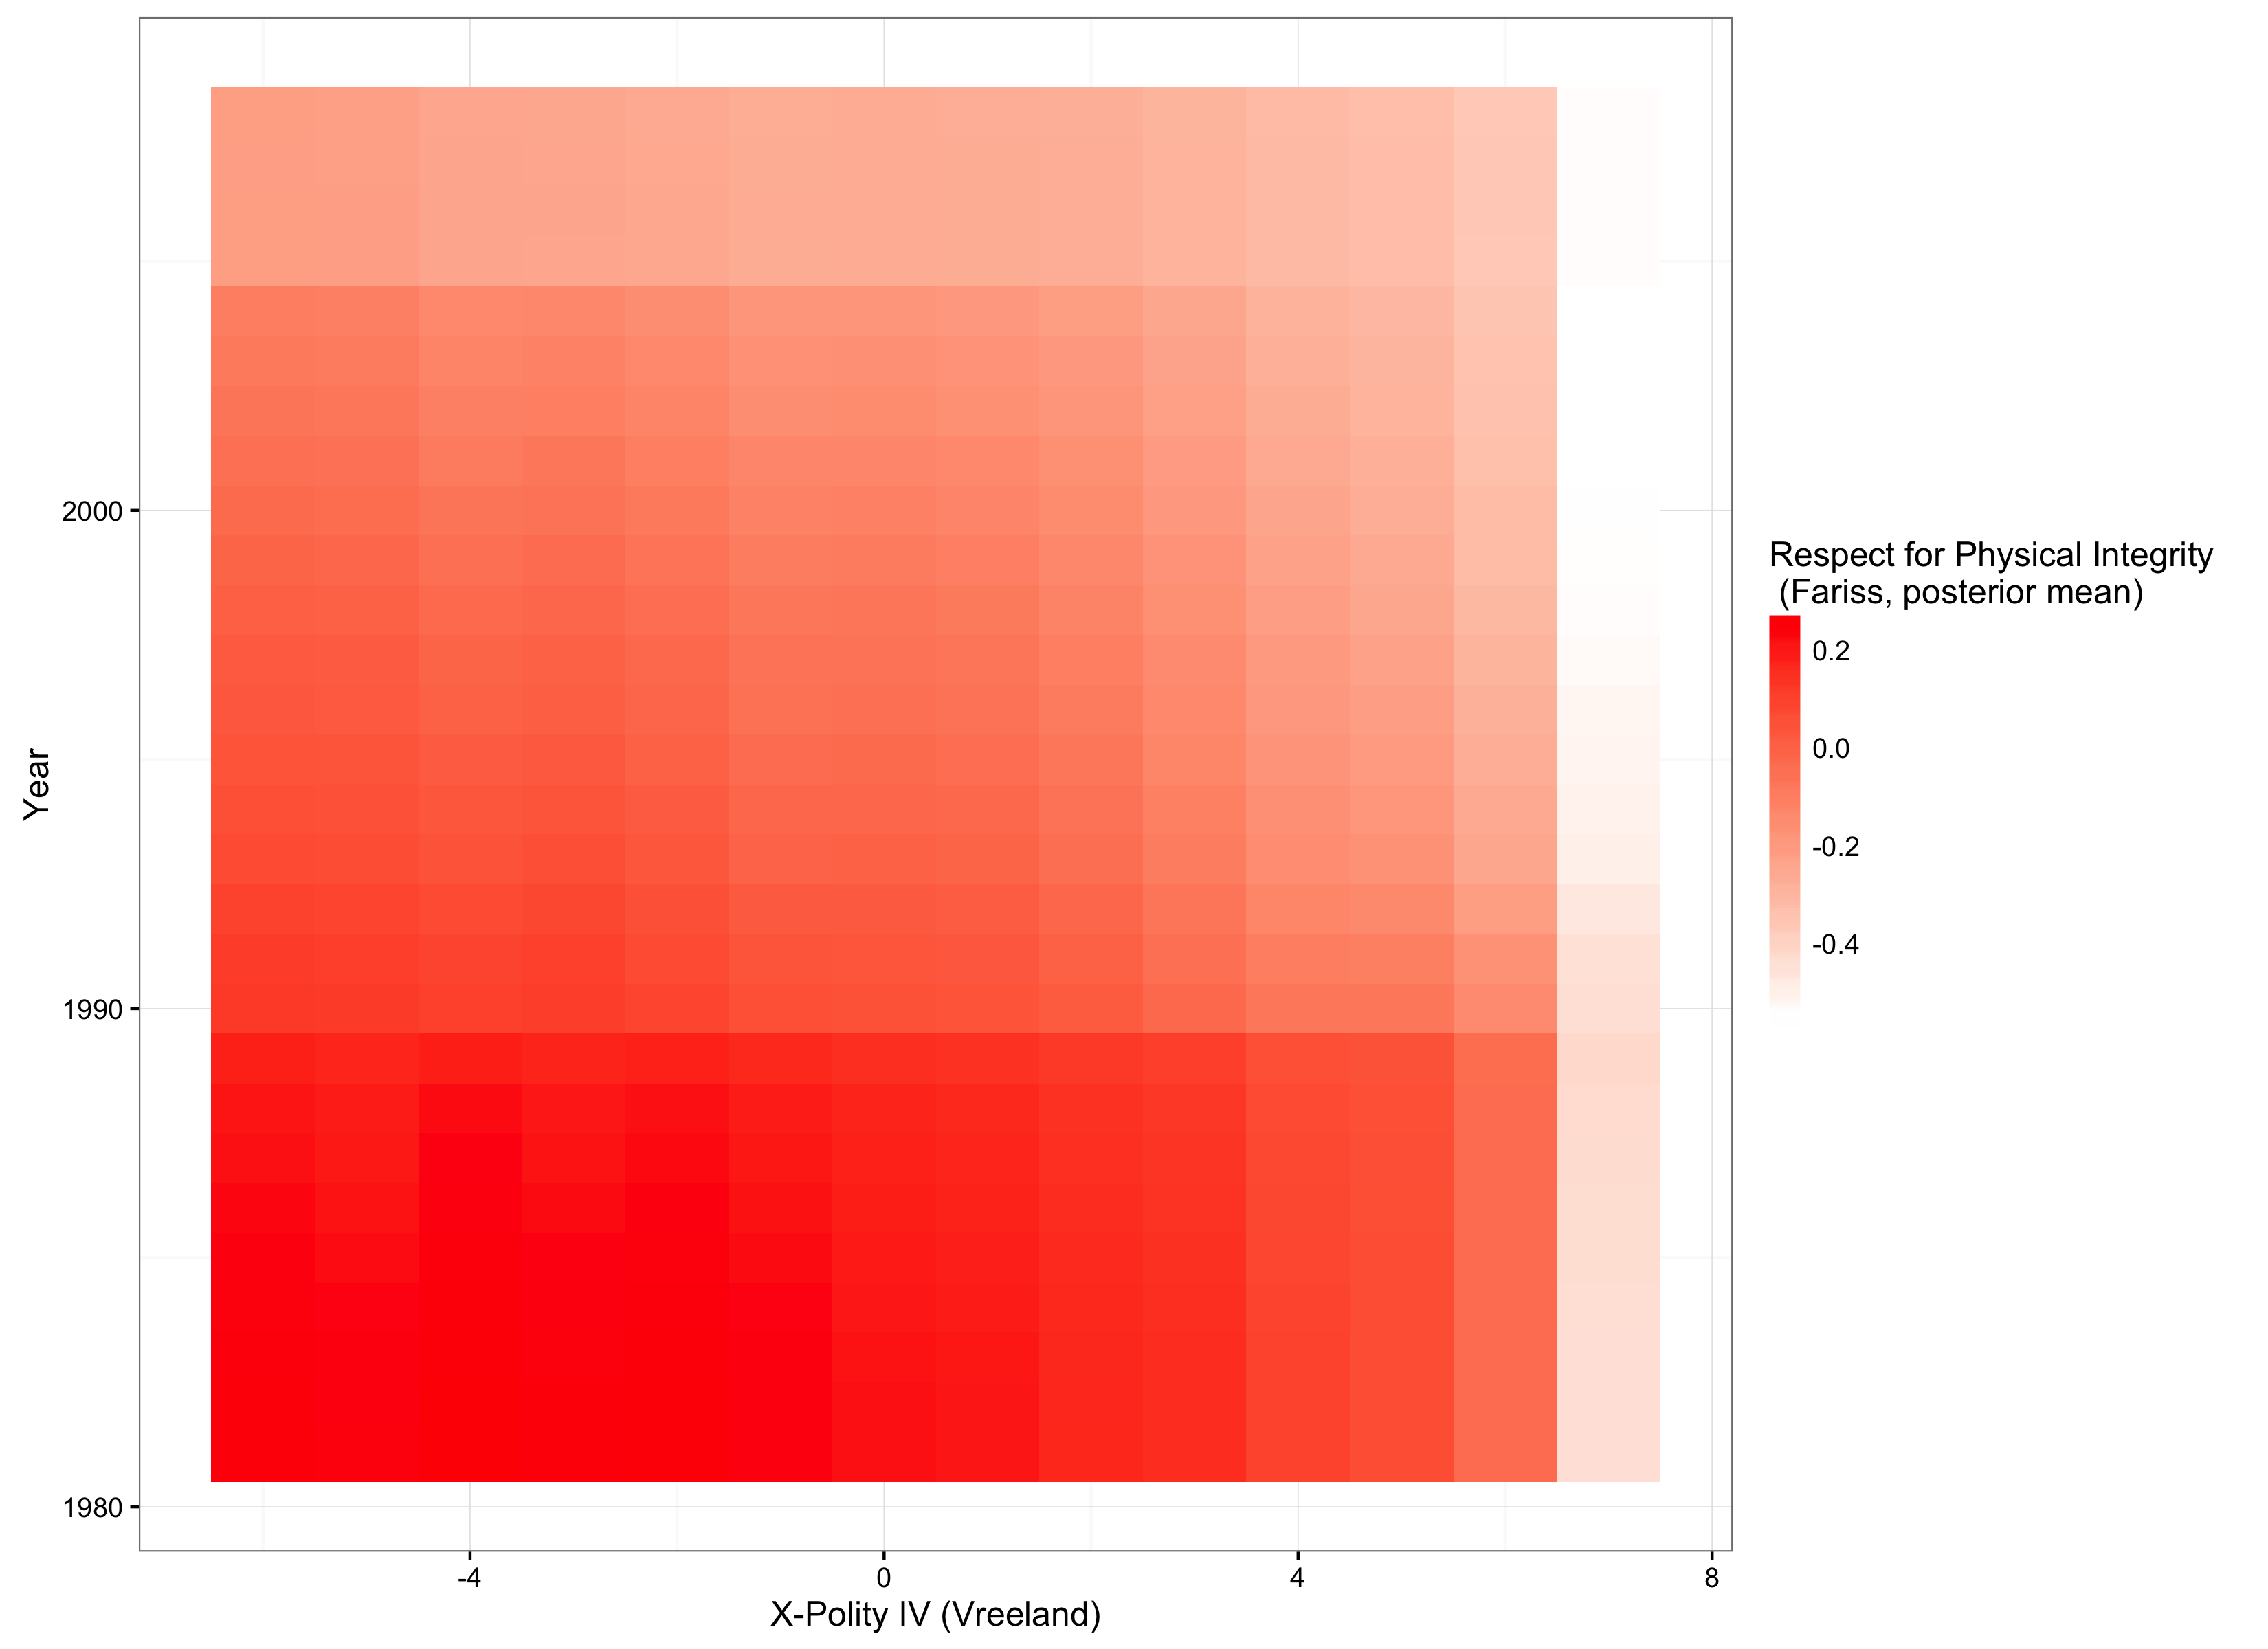
\includegraphics[width=100mm]{../figures/latent_mean_xpolity_nas_int_year_tile.png}
\end{center}
\caption{Partial dependence of X-Polity on Repression over Time.}
\label{xpolity_rep}
\end{figure}

\clearpage

\begin{figure}[ht!]
\begin{center}
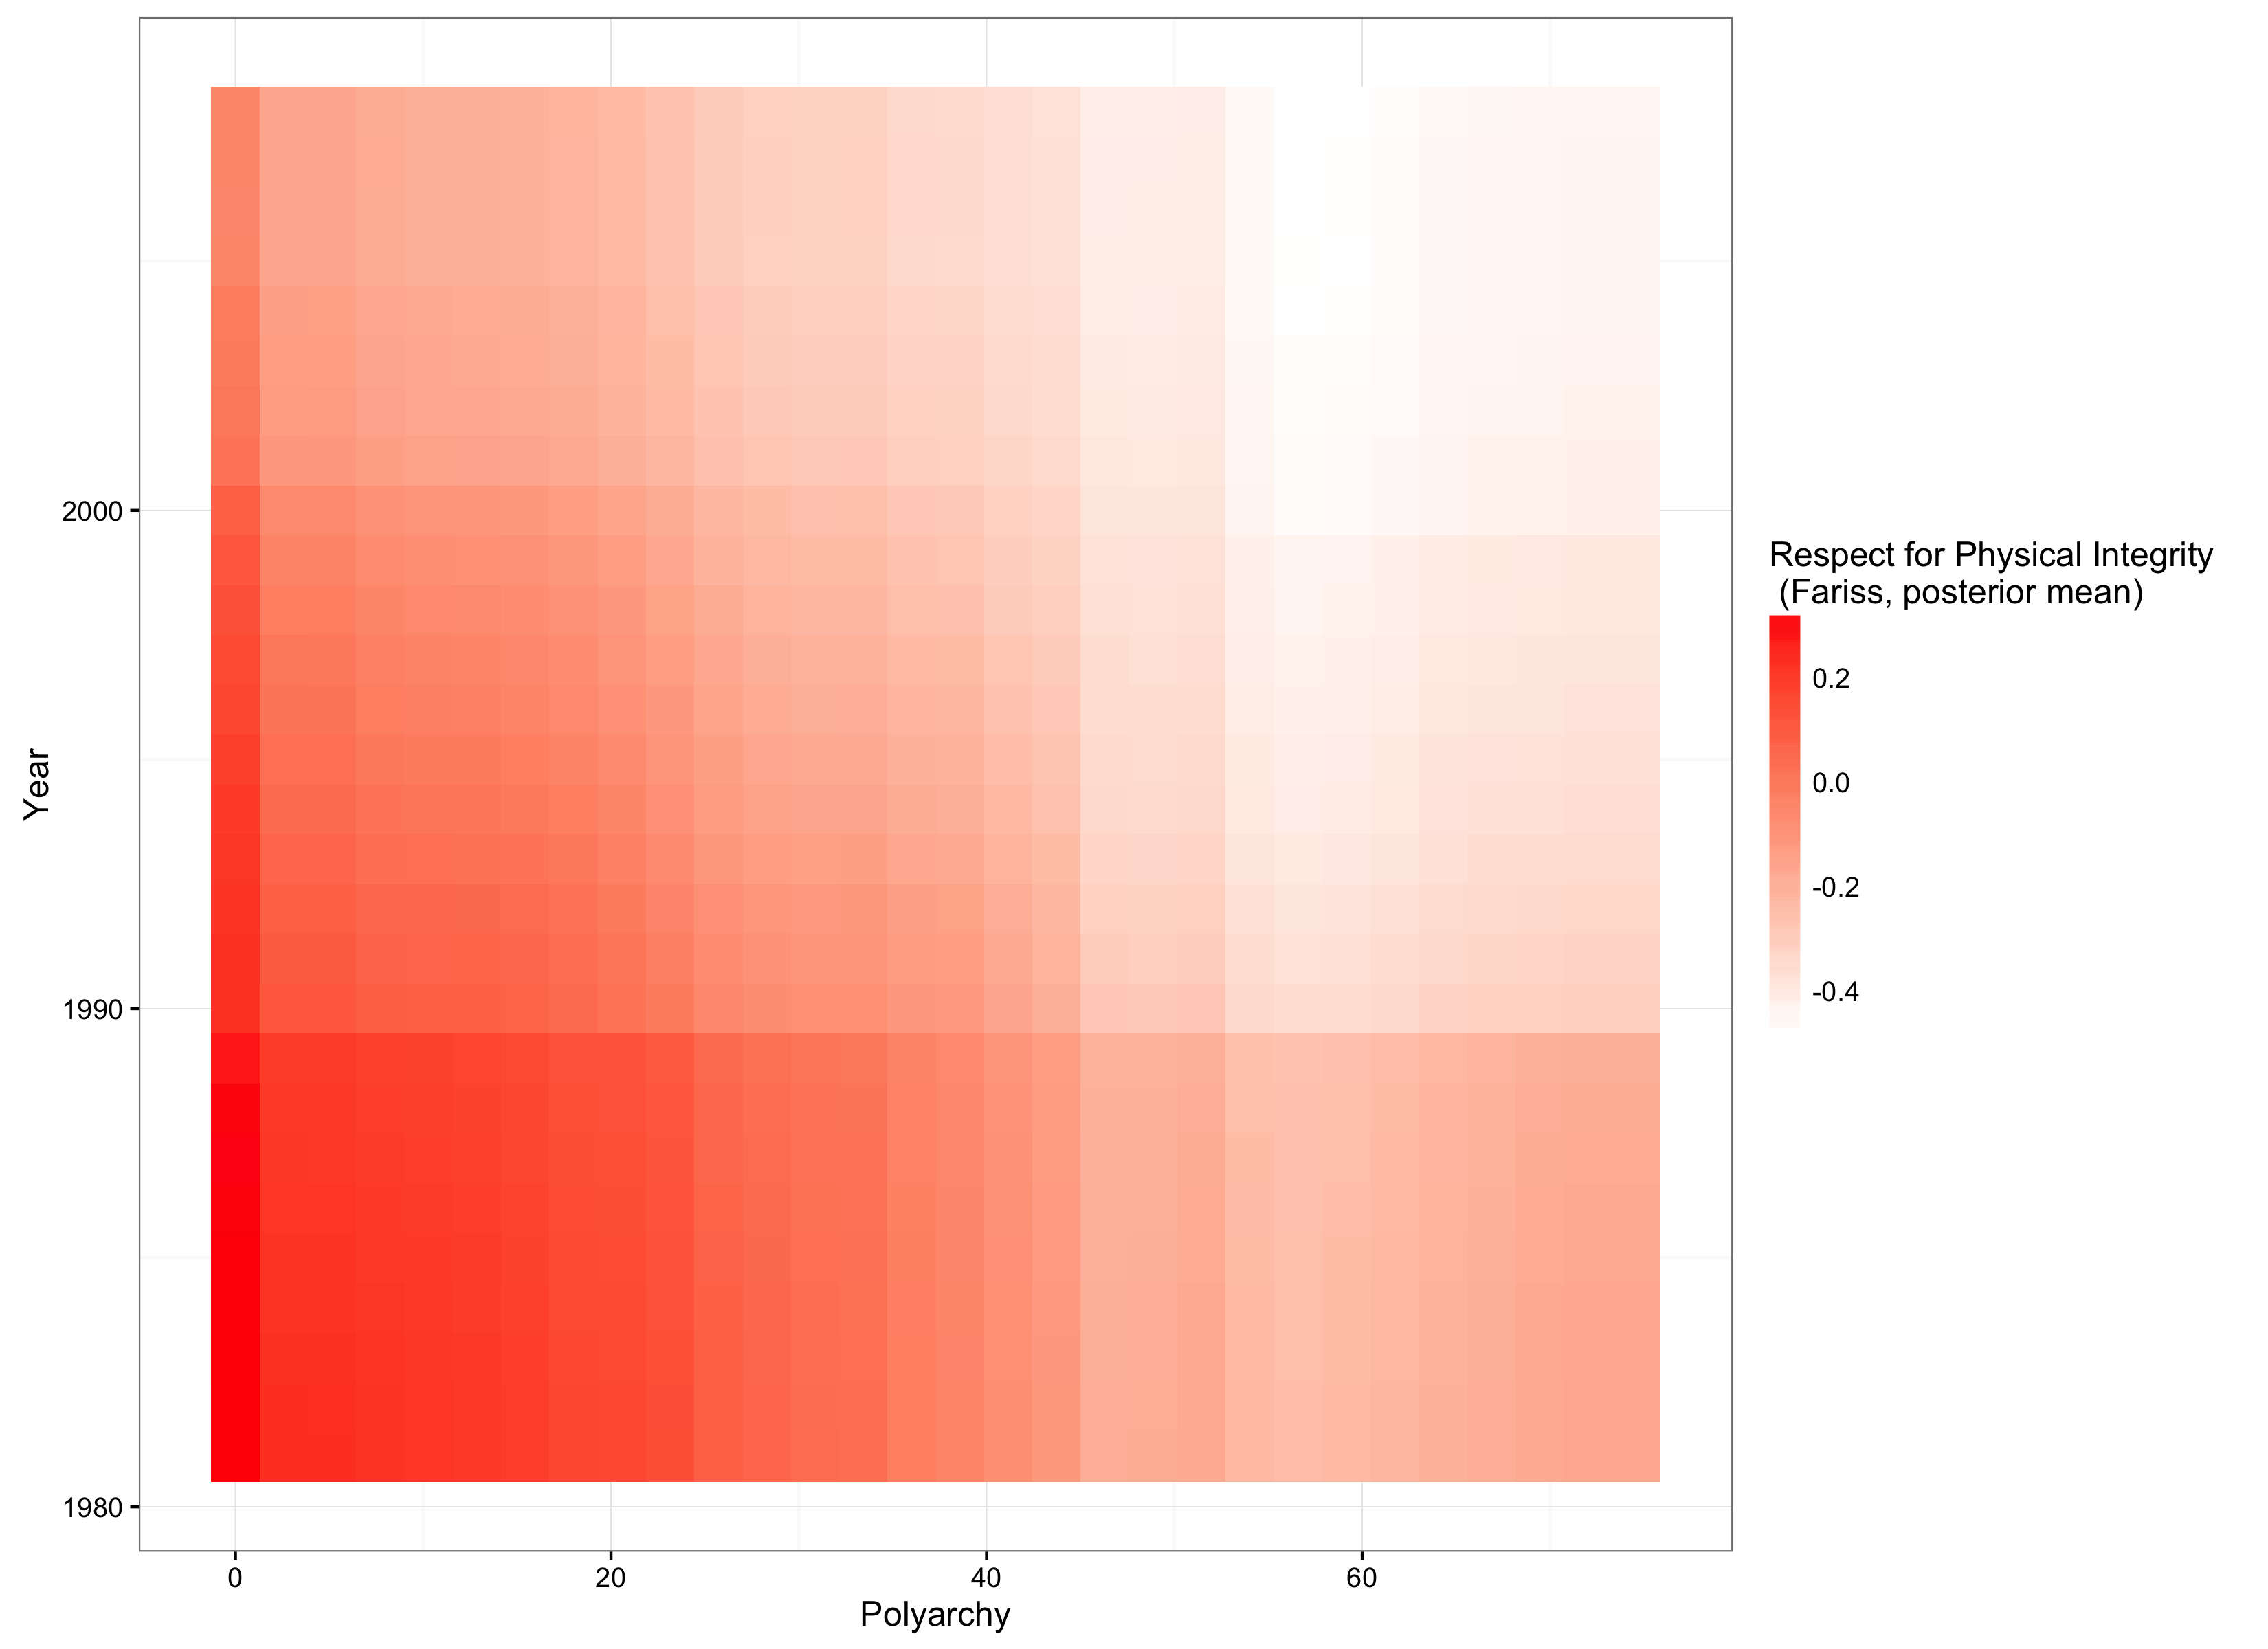
\includegraphics[width=100mm]{../figures/latent_mean_part_int_year_tile.png}
\end{center}
\caption{Partial dependence of Participation on Repression over Time.}
\label{part_rep}
\end{figure}

Figures \ref{xuds_terror}, \ref{xpolity_terror}, and \ref{part_terror} provide the heat maps of the risk of terrorism events from our models using X-UDS, X-Polity, and Polyarchy, respectively.  As with respect to civil conflict and repression, we find that important changes to these relationships occurred at the end of the Cold War, although a smaller shift also occurred in 1993.  Figure \ref{xuds} indicated support for the MVM Hypothesis using the X-UDS data, and Figure \ref{xuds_terror} provides additional evidence in support by indicating that the middle range of regime types had the largest risk of terror attacks through the years in our data.  Yet, while Figure \ref{part} indicated support for the MVM Hypothesis using the Polyarchy data, Figure \ref{part_terror} suggests this finding may be driven by Cold War-era data.  Since 1993, states with little or no electoral participation are about at the same level of risk for terror events as are states in the middle range.

\clearpage

\begin{figure}[ht!]
\begin{center}
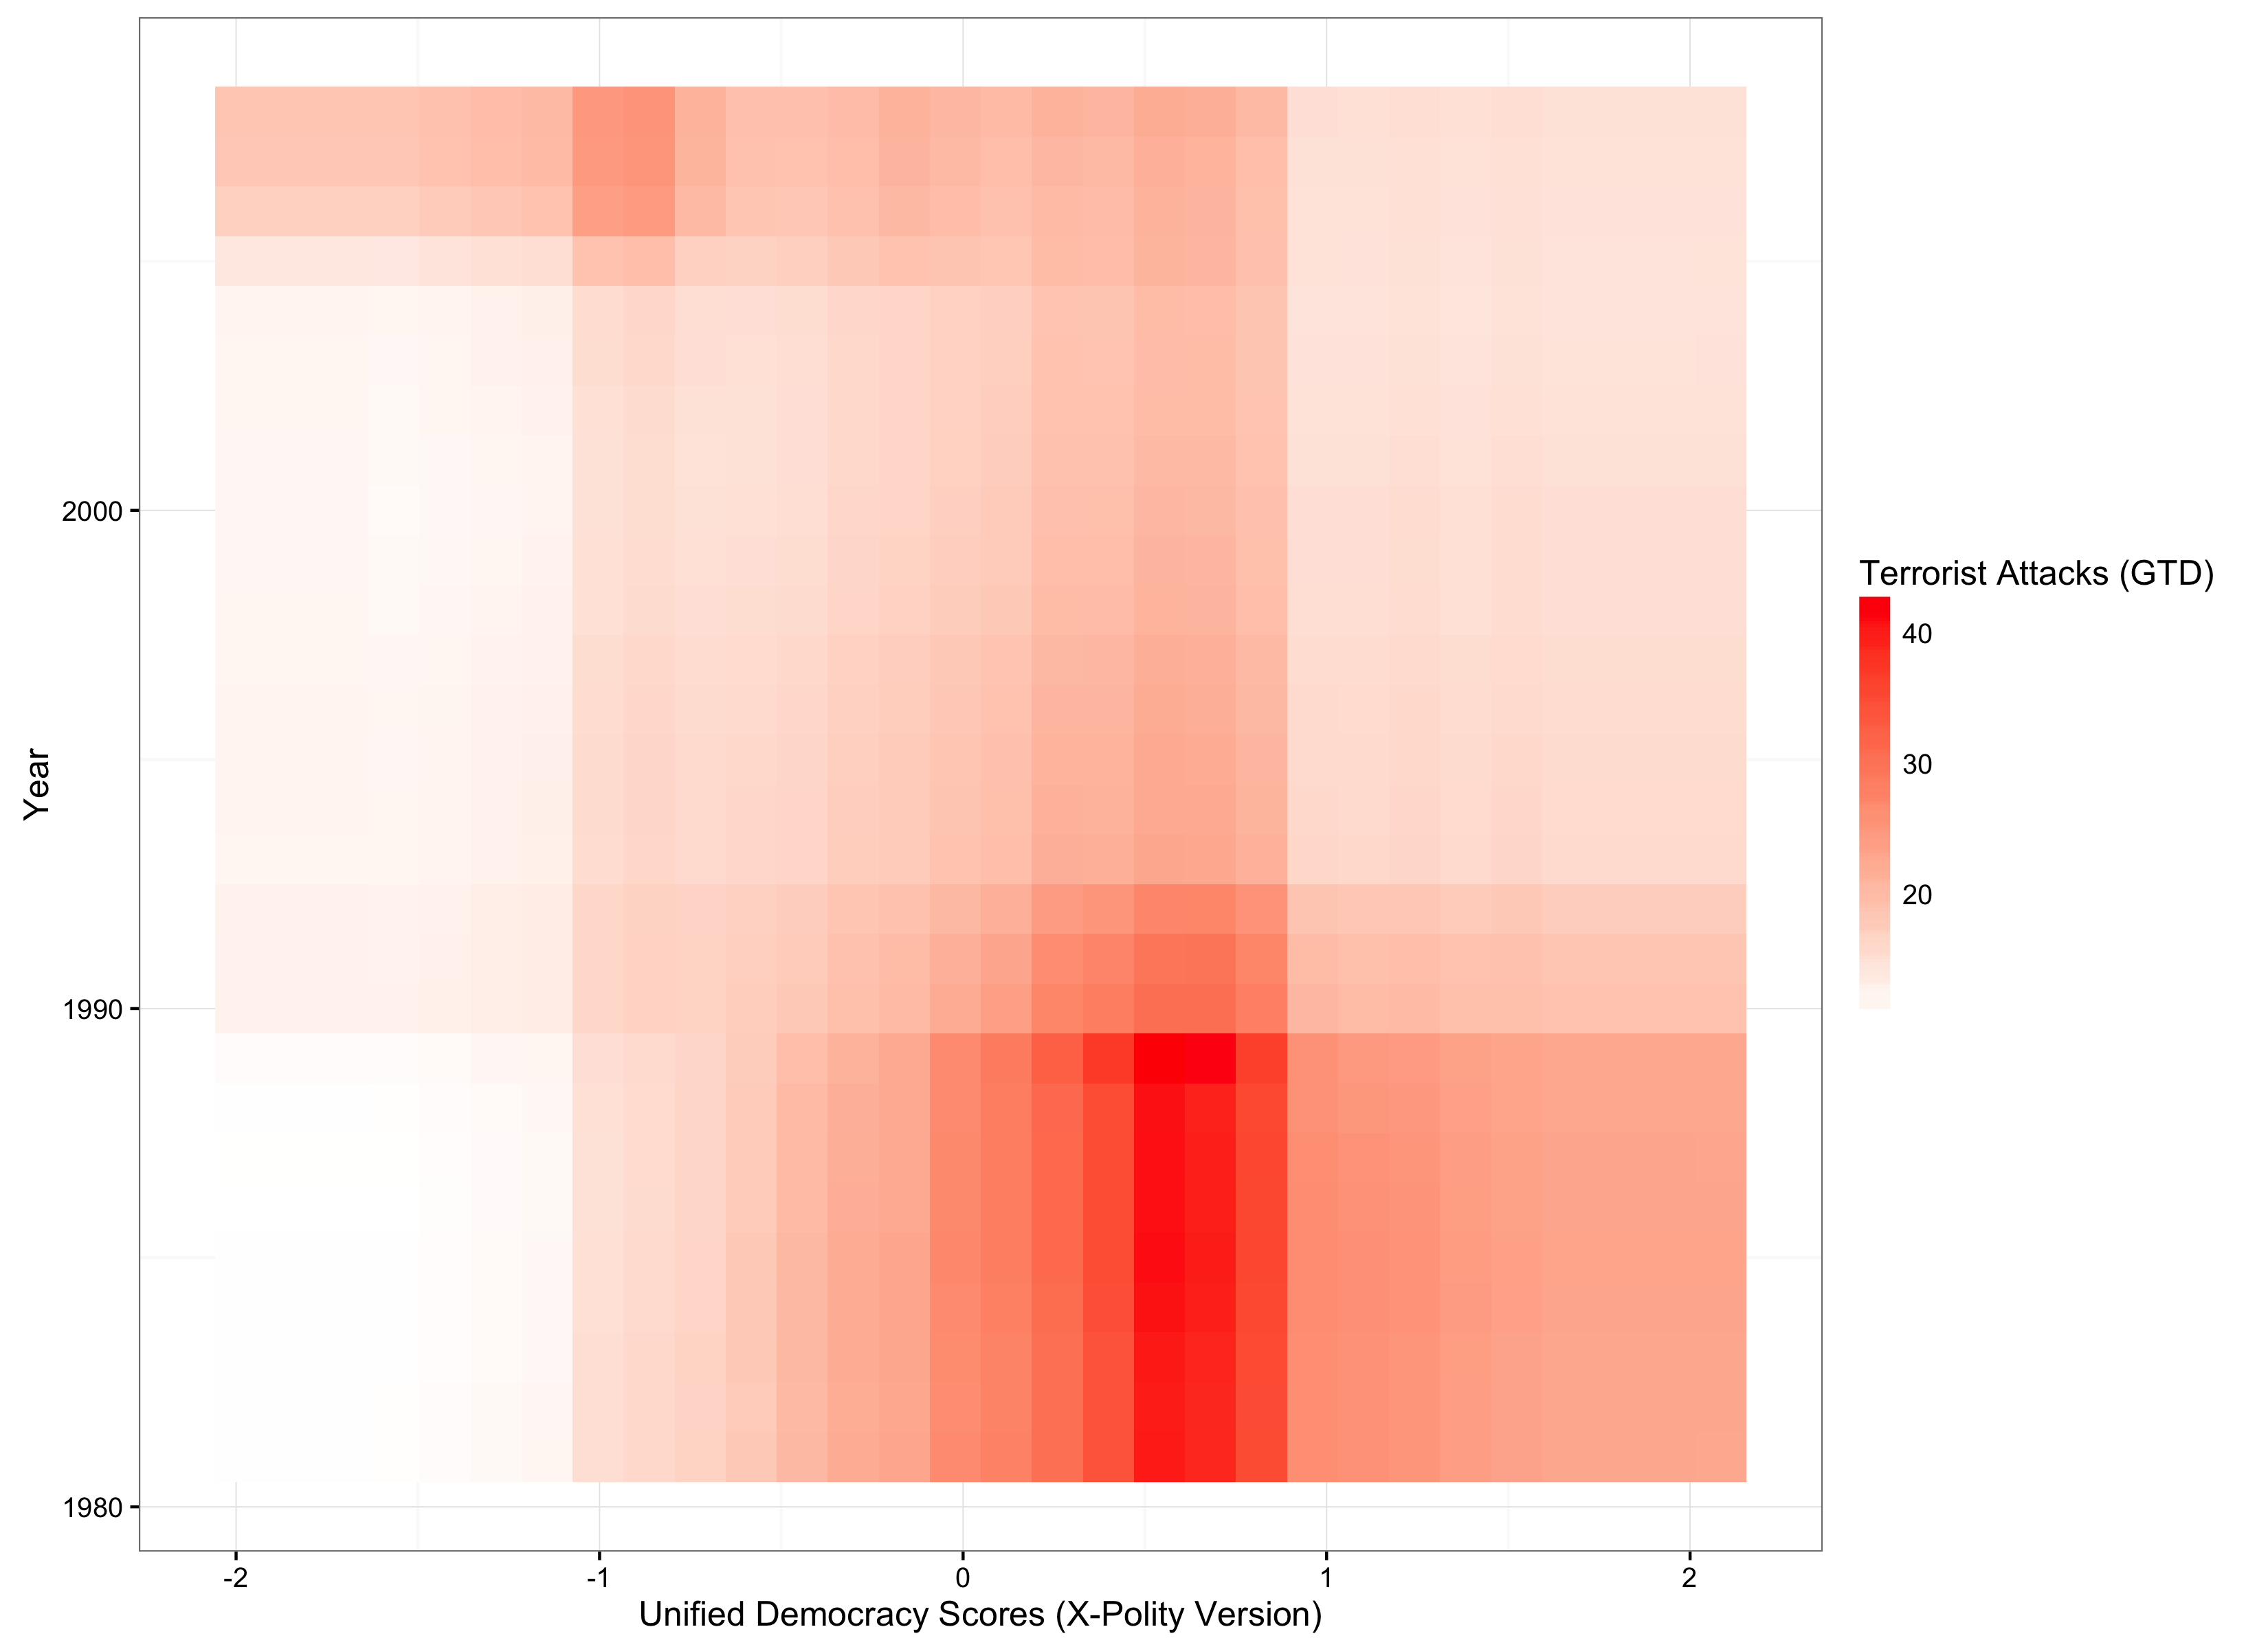
\includegraphics[width=100mm]{../figures/terror_events_uds_xpolity_int_year_tile.png}
\end{center}
\caption{Partial dependence of X-UDS on Terror Events over Time.}
\label{xuds_terror}
\end{figure}

\begin{figure}[h!]
\begin{center}
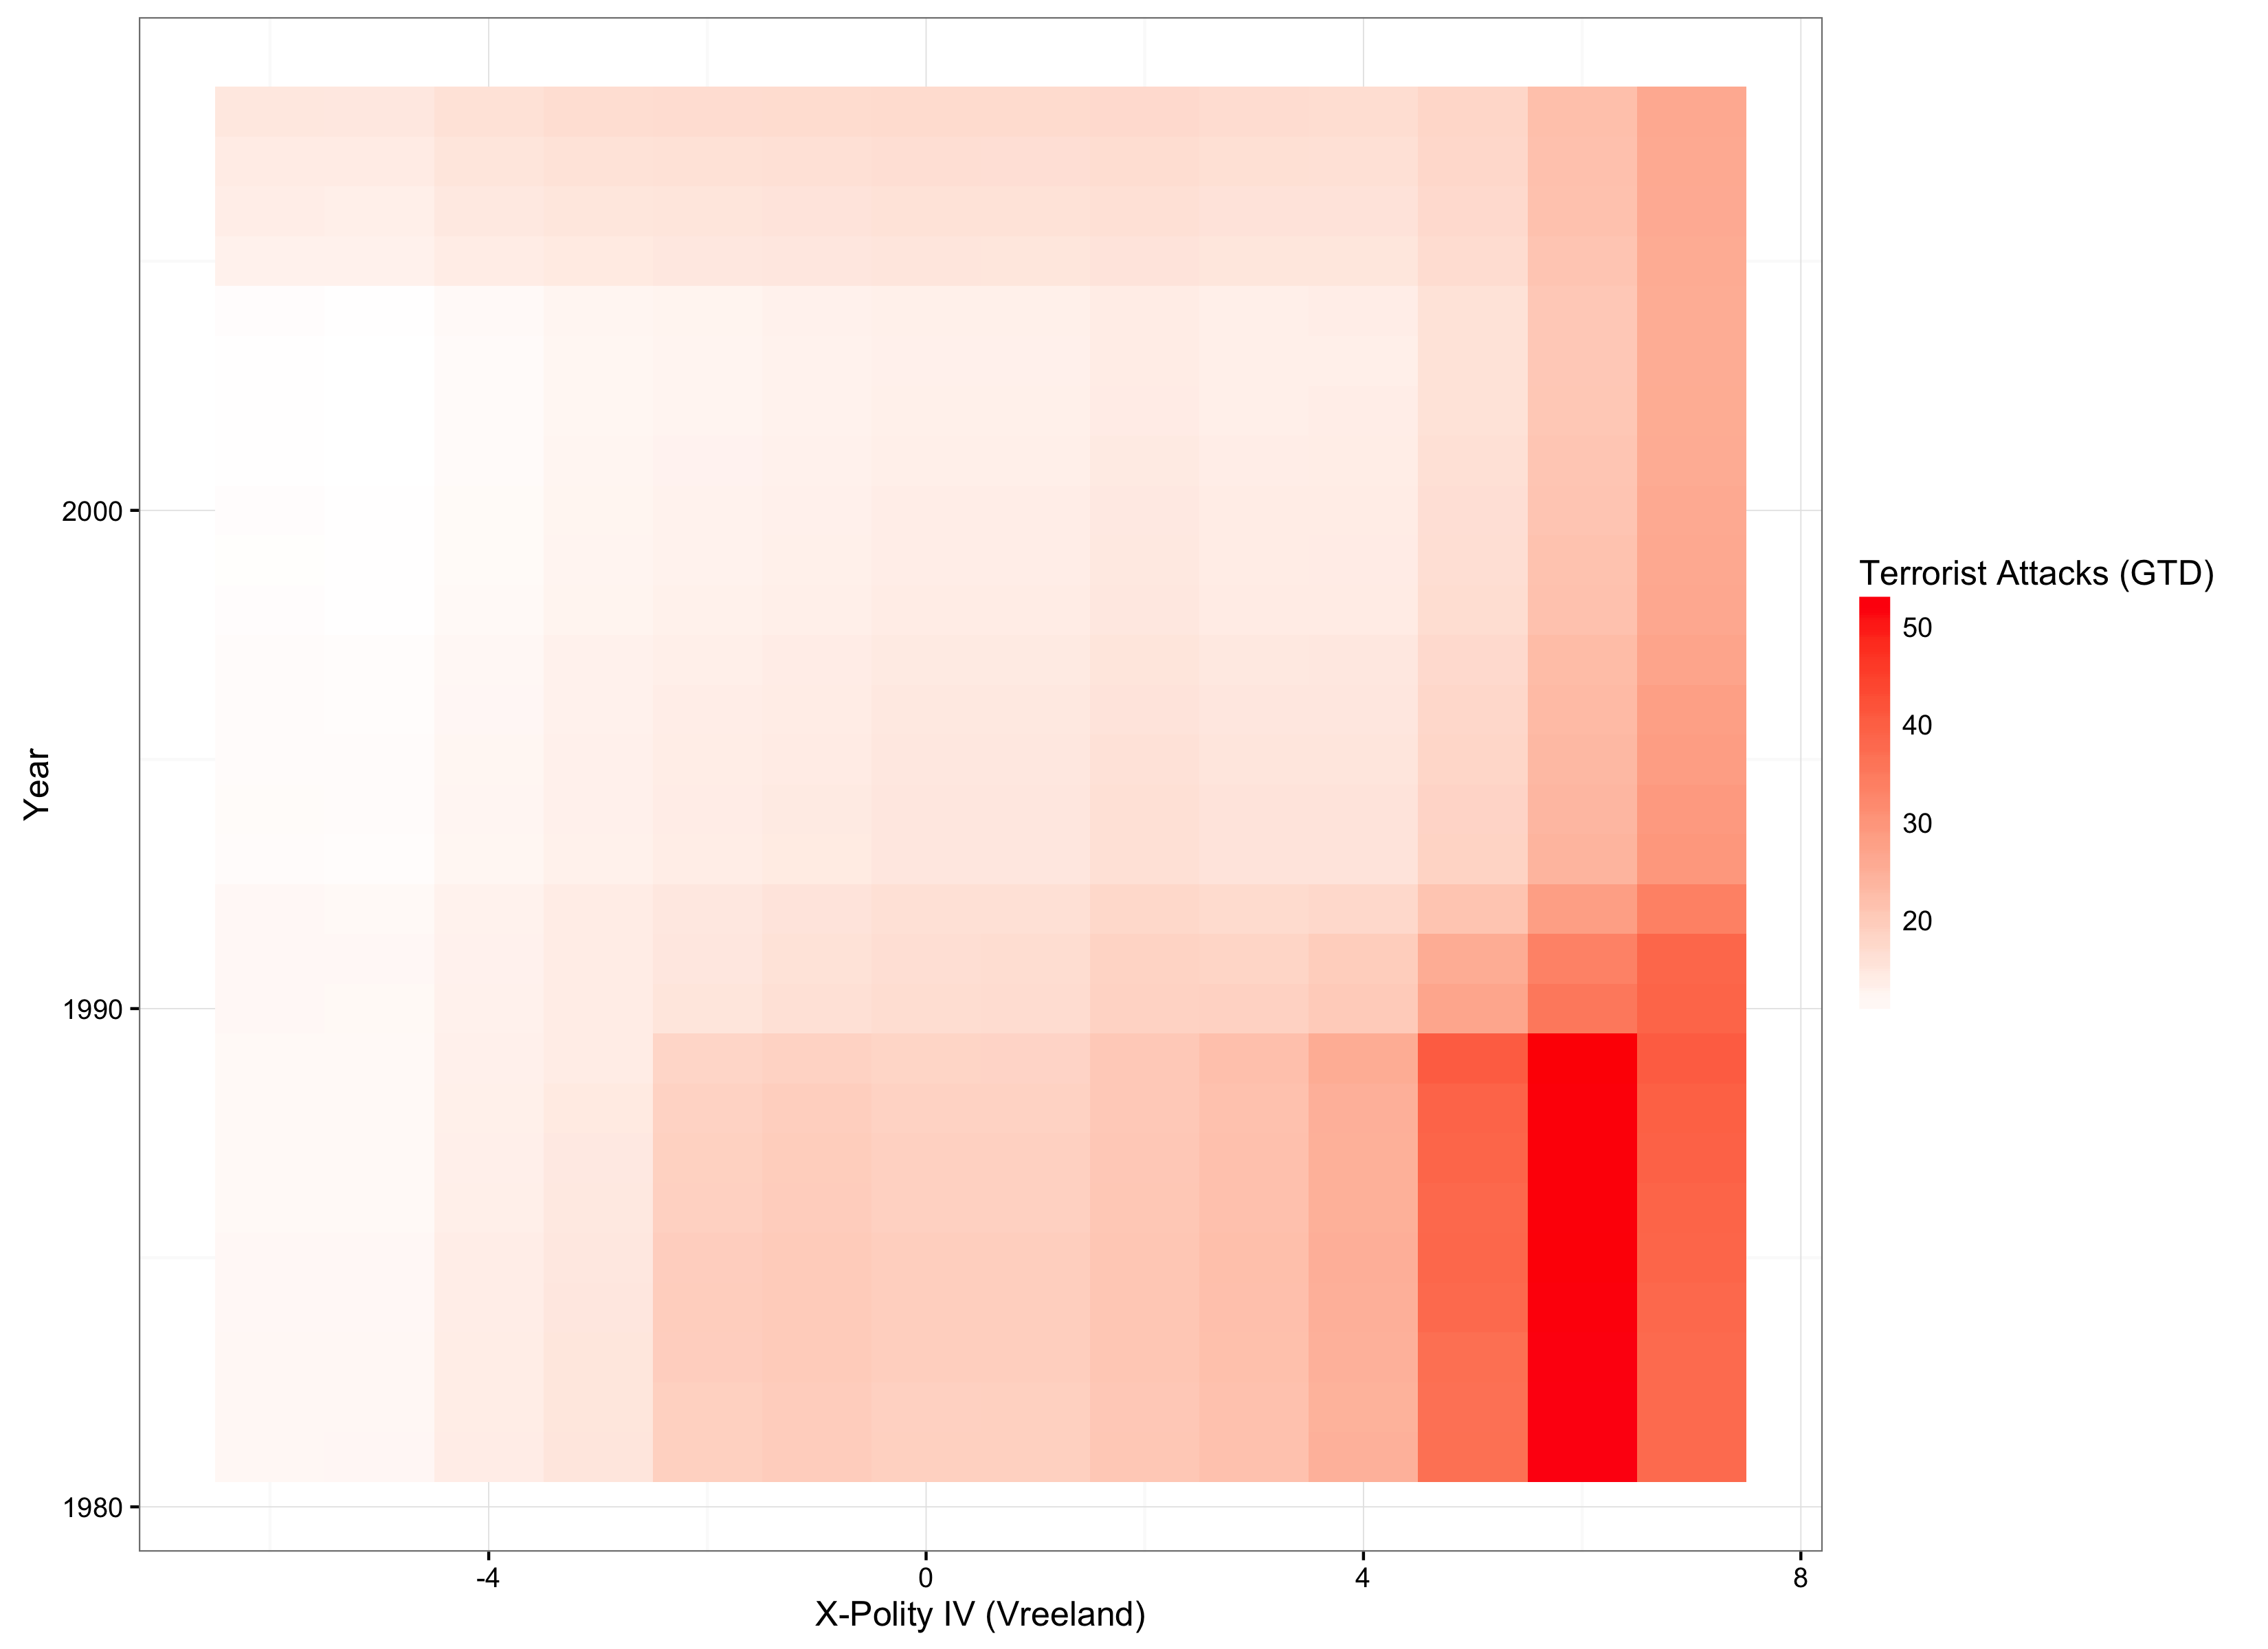
\includegraphics[width=100mm]{../figures/terror_events_xpolity_nas_int_year_tile.png}
\end{center}
\caption{Partial dependence of X-Polity and Terror Events over Time.}
\label{xpolity_terror}
\end{figure}

\clearpage

\begin{figure}[ht!]
\begin{center}
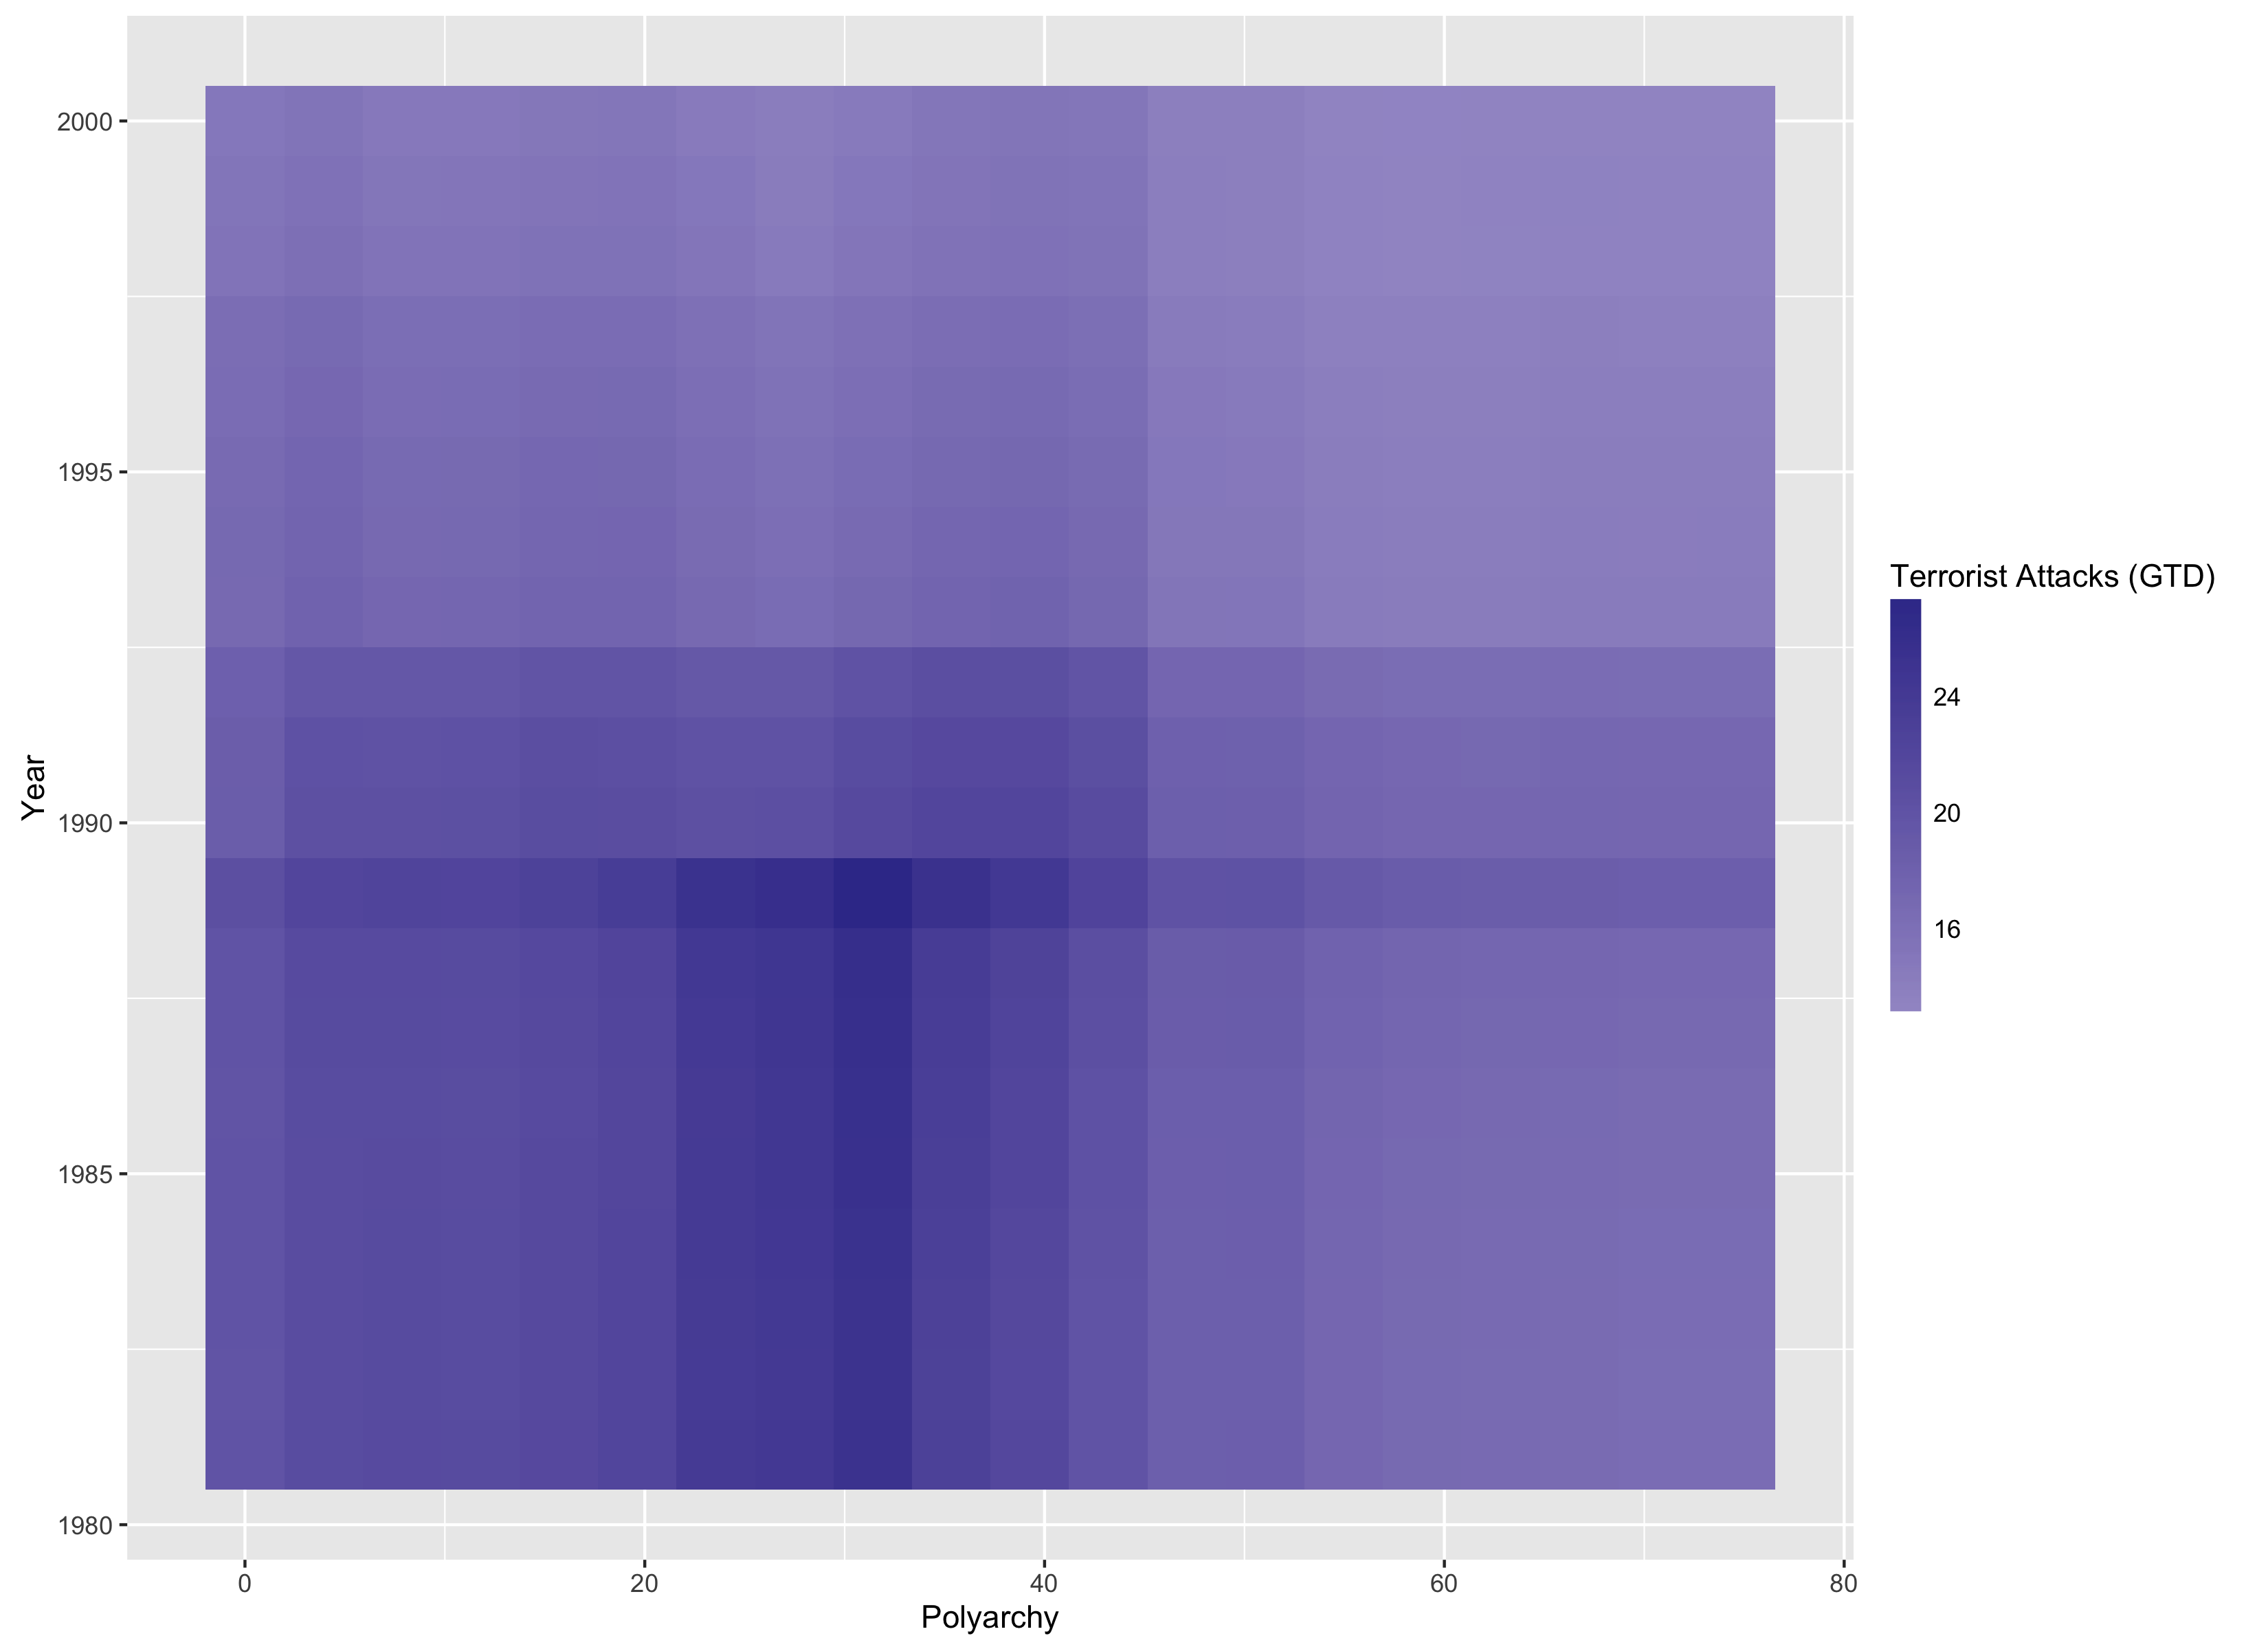
\includegraphics[width=100mm]{../figures/terror_events_part_int_year_tile.png}
\end{center}
\caption{Partial dependence of Participation and Terror Events over Time.}
\label{part_terror}
\end{figure}

\section{Conclusions}

In this section, we offer preliminary conclusions and implications, as well as describing the next steps we intend to take in developing this manuscript.  Our intent in this paper is to offer an improved research design for testing the MVM Hypothesis across space, time, forms of conflict, and measures of regime type. Our results indicate that support for the MVM Hypothesis depends, in part, on these factors.  With respect to the most commonly analyzed forms of conflict, we find relatively strong support for the MVM Hypothesis with respect to terrorism (2 out of 3 measures of regime type), limited support with respect to civil conflicts (1 out of 3), and no support with respect to the repression of physical integrity rights (0 out of 3).

As we continue to develop this manuscript, we plan to conduct several additional analyses.  First, we plan to disaggregate civil conflicts into types.  \citet{buhaug2006relative}, for example, argues that anocracies are more likely to experience civil conflicts in which rebels aim to control the government, but that this does not apply to conflict over territory.  We will further test this argument using the procedure outlined above.  Second, we plan to conduct additional analyses of missing data.  In some cases, missingness is informative so it may be advantageous to treat it as such. For example, the Polity data have a number of missingness categories that indicate whether the country in question is undergoing a regime transition, interregnum, or interruption. We utilize surrogate splitting to deal with this missingness, but we also plan treat the Polity IV variable as unordered, with the categories of missingness treated as a categorical predictor.  Third, we plan to more directly account for dynamic changes in regime type in our model.  Doing so will allow us to directly test whether democratizing states are more likely to experience conflict, as many have argued.

While we consider our current findings preliminary, they suggest several implications for our understanding of the relationship between regime type and conflict.  First, our results indicate that, with respect to several forms of conflict, whether or not we find support for the MVM Hypothesis depends on the measure of regime type used.  Our aim in this paper has been to be neutral regarding these measures rather than arguing for one measure over the others.  We hope scholars will build on our research by examining why it is the case that support for the MVM Hypothesis at times depends on the regime type measure.  It is likely the case, for example, that the Polyarchy participation measure captures a concept of democracy that differs from that captured by X-Polity.  Our findings therefore raise questions about how these concepts differ and why one might be associated with more violence in the middle range, while the other is not.

Second, the form of violence with respect to which we find the most support for the MVM Hypothesis is terrorism.  This is especially interesting because terrorism scholars have not focused on the concept of anocracy to the same extent as, for example, civil war scholars.  Instead, much new work on the relationship between regime type and terrorism focuses on specific institutions.  Our result is especially consistent with arguments such as those made by
\citet{aksoy2012terrorism} and \citet{aksoy2014electoral}, indicating that states with some democratic institutions may experience more terrorism, but that additional such institutions reduce this risk.  Our results suggest a similar pattern, but additional work is needed to determine which aspects of democracy contribute most to the inverse-U shape of our results.

Finally, our results indicate that the important changes have occurred over time.  Most importantly, we observe many structural changes in the data around the end of the Cold War.  This cannot simply be explained by a greater or lesser propensity toward certain conflict types during and after the Cold War.  Instead, it indicates that, in some way, the Cold War changed the relationship between regime type and conflict.  This question bears further investigation.  Why, for example, do our terrorism results based on the Polyarchy data support the MVM Hypothesis during the Cold War but not after?  Did the unleashing of nationalist agendas at the end of the Cold War affect the relationship between electoral participation and terrorism, and, if so, how?  In addition, why did the end of the Cold War change the relative risk of civil conflicts in many regime types (especially along the X-UDS and X-Polity scales)?  We hope our work will spur additional research into such questions.

\clearpage

\bibliographystyle{apsr}
\bibliography{references}

\end{document}